%% ============================================================
%%  TFG — Universidade de Santiago de Compostela
%%  Grao en Empresa e Tecnoloxía
%%
%%  Análise experimental da optimización de sistemas RAG
%%  mediante técnicas de recuperación e procesamento de contexto
%%
%%  Compilar con: pdflatex → biber → pdflatex → pdflatex
%% ============================================================

\documentclass[11pt, a4paper, oneside]{report}

%% ── Codificación e lingua ────────────────────────────────────
\usepackage[utf8]{inputenc}
\usepackage[T1]{fontenc}
\usepackage[galician]{babel}

%% ── Tipografía: Carlito (clon libre de Calibri) ──────────────
\usepackage[sfdefault]{carlito}
\usepackage{microtype}

%% ── Páxina ───────────────────────────────────────────────────
\usepackage[
  a4paper,
  top=2.5cm, bottom=2.5cm,
  left=3.0cm,  right=3.0cm,
  headheight=1.25cm,
  headsep=0.5cm,
  footskip=1.25cm
]{geometry}
\usepackage{setspace}
\onehalfspacing

%% ── Cabeceiras e pé de páxina ────────────────────────────────
\usepackage{fancyhdr}
\pagestyle{fancy}
\fancyhf{}
%% Cabeceira: título do traballo á dereita (Calibri 9 = fontsize 9)
\fancyhead[R]{\fontsize{9}{11}\selectfont
  Análise experimental da optimización de sistemas RAG}
%% Pé: autor á esquerda (9pt), nº de páxina á dereita (11pt)
\fancyfoot[L]{\fontsize{9}{11}\selectfont Roi Caride Borrajo}
\fancyfoot[R]{\fontsize{11}{13}\selectfont\thepage}
\renewcommand{\headrulewidth}{0.4pt}
\renewcommand{\footrulewidth}{0pt}
%% Páxinas de inicio de sección: mesmo formato que o resto (autor á esq., nº á dereita)
\fancypagestyle{plain}{%
  \fancyhf{}
  \fancyhead[R]{\fontsize{9}{11}\selectfont
    Análise experimental da optimización de sistemas RAG}
  \fancyfoot[L]{\fontsize{9}{11}\selectfont Roi Caride Borrajo}
  \fancyfoot[R]{\fontsize{11}{13}\selectfont\thepage}
  \renewcommand{\headrulewidth}{0.4pt}
}

%% ── Gráficos e táboas ────────────────────────────────────────
\usepackage{graphicx}
\usepackage{float}
\usepackage{booktabs}
\usepackage{longtable}
\usepackage{array}
\usepackage{multirow}
\usepackage{caption}
\usepackage{subcaption}
\usepackage{tikz}
\usetikzlibrary{arrows.meta, positioning, fit, backgrounds, calc}
\usepackage[table]{xcolor}

%% Formato de títulos de táboas/figuras: Calibri 11 normal centrado
\captionsetup{
  font={normalsize},
  labelfont={normalfont},
  justification=centering,
  position=above
}
%% Etiqueta das táboas como "Táboa" (coherente co texto; babel galego usa "Cadro")
\addto\captionsgalician{\renewcommand{\tablename}{Táboa}}

%% ── Notas a rodapé: Calibri 8, interliñado sinxelo ──────────
\makeatletter
\long\def\@makefntext#1{%
  \parindent 1em\noindent
  \hb@xt@1.8em{\hss\@makefnmark}%
  \fontsize{8}{9.6}\selectfont #1}
\makeatother

%% ── Matemáticas ──────────────────────────────────────────────
\usepackage{amsmath}
\usepackage{amssymb}
\usepackage{bm}


%% ── Hiperligazóns ────────────────────────────────────────────
\usepackage[
  colorlinks=true,
  linkcolor=black,
  citecolor=blue!70!black,
  urlcolor=blue!70!black,
  pdfview=FitH,
  pdftitle={Análise experimental da optimización de sistemas RAG},
  pdfauthor={Roi Caride Borrajo},
  pdfsubject={TFG — Grao en Empresa e Tecnoloxía, USC}
]{hyperref}
\usepackage{xurl}
\usepackage{csquotes}
\Urlmuskip=0mu plus 1mu\relax
\setlength{\emergencystretch}{3em}

%% ── Bibliografía (estilo autor-ano, formato APA) ─────────────
\usepackage[
  backend=biber,
  style=authoryear,
  sorting=nyt,
  natbib=true,
  maxbibnames=6,
  minbibnames=3,
  maxcitenames=2,
  backref=false
]{biblatex}
\addbibresource{referencias.bib}

%% Coma entre autor e ano nas citas: (Autor, ano) — esixido pola guía
\renewcommand*{\nameyeardelim}{\addcomma\space}

%% Espazo e liña separadora entre entradas da bibliografía
\newcounter{bibitemctr}
\defbibenvironment{bibliography}
  {\list{}
    {\setlength{\leftmargin}{\bibhang}%
     \setlength{\itemindent}{-\leftmargin}%
     \setlength{\itemsep}{0pt}%
     \setlength{\parsep}{0pt}}%
   \setcounter{bibitemctr}{0}}
  {\endlist}
  {\stepcounter{bibitemctr}%
   \ifnum\value{bibitemctr}>1
     \bigskip{\color{gray!40}\hrule height 0.4pt}\smallskip
   \fi
   \item}

%% ── Acrónimos ────────────────────────────────────────────────
\usepackage[nohyperlinks]{acronym}

%% ── Outros ───────────────────────────────────────────────────
\usepackage{pdfpages}
\usepackage{enumitem}
\usepackage{titlesec}
\usepackage{tocloft}
\usepackage{xspace}

\makeatletter
\AtBeginDocument{%
  \renewcommand{\labelenumi}{\theenumi.}%
  \renewcommand{\labelenumii}{(\theenumii)}%
  \renewcommand{\labelenumiii}{\theenumiii.}%
  \renewcommand{\labelenumiv}{\theenumiv.}%
  \renewcommand{\labelitemi}{\textbullet}%
  \renewcommand{\labelitemii}{\normalfont\bfseries \textendash}%
  \renewcommand{\labelitemiii}{\textasteriskcentered}%
  \renewcommand{\labelitemiv}{\textperiodcentered}%
  \renewcommand{\@roman}[1]{\romannumeral#1}%
  \let\gl@roman\@roman
}
\makeatother

%% ── Formato de títulos ───────────────────────────────────────
%% Capítulos sen numerar (Introdución, Desenvolvemento, Conclusións...)
\titleformat{\chapter}[hang]
  {\normalfont\fontsize{18}{22}\bfseries}
  {}{0pt}{}
\titlespacing*{\chapter}{0pt}{0pt}{20pt}

%% Seccións (1. Título principal) — Calibri 16 negriña
\titleformat{\section}[hang]
  {\normalfont\fontsize{16}{20}\bfseries}
  {\thesection.}{0.5em}{}
\titlespacing*{\section}{0pt}{18pt}{10pt}

%% Subseccións (1.1. Subtítulo) — Calibri 14 negriña
\titleformat{\subsection}[hang]
  {\normalfont\fontsize{14}{18}\bfseries}
  {\thesubsection.}{0.5em}{}
\titlespacing*{\subsection}{0pt}{14pt}{6pt}

%% Subsubseccións (1.1.1. Subtítulo de segunda orde) — Calibri 14 normal
\titleformat{\subsubsection}[hang]
  {\normalfont\fontsize{14}{18}\mdseries}
  {\thesubsubsection.}{0.5em}{}
\titlespacing*{\subsubsection}{0pt}{12pt}{4pt}

%% Numeración de seccións independente do capítulo (1., 1.1., 1.1.1.)
\renewcommand{\thesection}{\arabic{section}}
\renewcommand{\thesubsection}{\thesection.\arabic{subsection}}
\renewcommand{\thesubsubsection}{\thesubsection.\arabic{subsubsection}}
\setcounter{secnumdepth}{3}  %% numerar tamén os subsubsections (1.1.1)

%% ── Sangría de primeira liña ─────────────────────────────────
\usepackage{indentfirst}
\setlength{\parindent}{1.25cm}

%% ── Comandos propios ─────────────────────────────────────────
\newcommand{\rag}{\textsc{rag}\xspace}
\newcommand{\llm}{\textsc{llm}\xspace}

%% Fonte debaixo de táboas e figuras (Calibri 9, centrada) — esixido pola guía
\newcommand{\fonte}[1]{%
  \par\smallskip
  {\centering\fontsize{9}{11}\selectfont Fonte: #1\par}}

%% ============================================================
\begin{document}

%% ── Numeración romana para páxinas preliminares ──────────────
\pagenumbering{roman}

%% ============================================================
%%  PORTADA  (modelo Anexo I — versión galega)
%% ============================================================
\hypersetup{pageanchor=false}
\begin{titlepage}
  \thispagestyle{empty}
  \centering

  %% Logo USC — substitúe usc_logo.png polo ficheiro oficial
  %% \includegraphics[width=0.28\textwidth]{usc_logo.png}\par
  \vspace*{1cm}

  {\large\bfseries Facultade de Administración e Dirección de Empresas\par}

  \vspace{2.5cm}

  %% Caixa de dúas columnas: esquerda = tipo de traballo, dereita = título
  \noindent
  \begin{tabular}{p{0.28\textwidth} | p{0.60\textwidth}}
    \parbox[t]{\linewidth}{\large\bfseries Traballo de\\[4pt] Fin de Grao} &
    {\fontsize{22}{28}\selectfont
      Análise experimental da optimización de sistemas RAG
      mediante técnicas de recuperación e procesamento de contexto}\\[16pt]
    & {\normalsize Roi Caride Borrajo}
  \end{tabular}

  \vspace{2.5cm}

  {\large Maio 2026\par}

  \vfill

  {\small
    Traballo de Fin de Grao presentado na Facultade de Administración e
    Dirección de Empresas da Universidade de Santiago de Compostela para
    a obtención do Grao en Empresa e Tecnoloxía\par}
\end{titlepage}
\hypersetup{pageanchor=true}

%% ============================================================
%%  RESUMO  (páxina 2 — máx. 300 palabras)
%% ============================================================
\chapter*{Resumo}
\addcontentsline{toc}{chapter}{Resumo}
\markboth{Resumo}{Resumo}

Os sistemas de \textit{Retrieval-Augmented Generation} (RAG) emerxeron como un dos
paradigmas máis prometedores para dotar os modelos de linguaxe de gran escala de
coñecemento factual actualizado e verificable. Ao integrar un módulo de recuperación
de información sobre fontes externas, os sistemas RAG mitigan dúas das limitacións
máis críticas dos LLM: a tendencia a xerar contido incorrecto (alucinación) e a
obsolescencia do coñecemento derivada do corte temporal do adestramento.

Non obstante, o rendemento dun sistema RAG non depende unicamente da capacidade xerativa
do modelo de linguaxe, senón en igual ou maior medida das decisións de deseño en cada
etapa da pipeline: que modelo de embedding se usa para a indexación, como se segmentan
os documentos, cales son os mecanismos de recuperación e como se filtra o contexto
antes de ser entregado ao xerador.

Este traballo presenta unha análise experimental sistemática mediante un deseño de
ablación secuencial en cinco fases: (0) establecemento dunha liña base, (1) comparativa
de modelos de embedding, (2) comparativa de estratexias de segmentación, (3) comparativa
de técnicas de retrieval incluíndo recuperación híbrida, (4) avaliación de técnicas de
expansión de consultas (HyDE, reescrita, multi-query, RAG-Fusion, entre outras) e (5)
avaliación de reranking pos-recuperación. O corpus está composto por documentos xurídicos
reais procedentes de EUR-Lex, e o rendemento mídese con seis métricas do framework RAGAS:
context recall, context precision, context entity recall, noise sensitivity, faithfulness
e response relevancy. O traballo achega dous resultados complementarios: a configuración
empírica óptima para o dominio xurídico e, sobre todo, un \textbf{marco experimental
reproducible} que permite determinar a configuración axeitada de calquera sistema RAG no
seu propio dominio, un activo metodolóxico de aplicabilidade directa en contornos
profesionais.

\vspace{1em}
\noindent\textbf{Palabras clave:} RAG, modelos de linguaxe de gran escala, recuperación de
información, embeddings, chunking, retrieval híbrido, reranking, HyDE, EUR-Lex, RAGAS.

\noindent\textbf{Número de palabras:} 10.630

\clearpage

%% ── Abstract (inglés) ────────────────────────────────────────
\chapter*{Abstract}
\addcontentsline{toc}{chapter}{Abstract}
\markboth{Abstract}{Abstract}

Retrieval-Augmented Generation (RAG) systems have emerged as one of the most promising
paradigms for equipping large language models with up-to-date and verifiable factual
knowledge. By integrating an information retrieval module over external sources, RAG
systems mitigate two critical limitations of LLMs: the tendency to generate incorrect
content (hallucination) and knowledge obsolescence derived from the training data cut-off.

However, the performance of a RAG system depends not only on the generative capability of
the language model but equally on design decisions at each stage of the pipeline: which
embedding model is used for indexing, how documents are segmented, what retrieval
mechanisms are employed, and how context is filtered before being delivered to the
generator.

This work presents a systematic experimental analysis through a sequential ablation design
in five optimization phases over an honest baseline: (1) a comparison of embedding models,
(2) a comparison of chunking strategies, (3) a comparison of retrieval techniques including
hybrid retrieval, (4) an evaluation of query expansion techniques (HyDE, rewriting,
multi-query, RAG-Fusion, among others), and (5) an evaluation of post-retrieval reranking;
the resulting pipeline is finally validated against a state-of-the-art stack from the
literature. The corpus consists of real legal documents from EUR-Lex, and performance is
measured with six RAGAS metrics: context recall, context precision, context entity recall,
noise sensitivity, faithfulness, and response relevancy. This work delivers two
complementary contributions: the empirically optimal configuration for the legal domain
and, above all, a \textbf{reproducible experimental framework} that enables determining the
right configuration of any RAG system in its own domain, a methodological asset of direct
applicability in professional settings.

\vspace{1em}
\noindent\textbf{Keywords:} RAG, large language models, information retrieval, embeddings,
chunking, hybrid retrieval, reranking, HyDE, EUR-Lex, RAGAS.

\clearpage

%% ============================================================
%%  ÍNDICE DE CONTIDOS
%% ============================================================
\tableofcontents
\clearpage

%% ============================================================
%%  ÍNDICE DE ABREVIATURAS
%% ============================================================
\chapter*{Índice de abreviaturas}
\addcontentsline{toc}{chapter}{Índice de abreviaturas}
\markboth{Índice de abreviaturas}{Índice de abreviaturas}

\begin{acronym}[NDCG]
  \acro{RAG}  {Retrieval-Augmented Generation}
  \acro{LLM}  {Large Language Model}
  \acro{NLP}  {Natural Language Processing}
  \acro{IR}   {Information Retrieval}
  \acro{QA}   {Question Answering}
  \acro{API}  {Application Programming Interface}
  \acro{EU}   {European Union}
  \acro{MRR}  {Mean Reciprocal Rank}
  \acro{NDCG} {Normalized Discounted Cumulative Gain}
  \acro{HyDE} {Hypothetical Document Embeddings}
  \acro{MMR}  {Maximal Marginal Relevance}
  \acro{DPR}  {Dense Passage Retrieval}
  \acro{BERT} {Bidirectional Encoder Representations from Transformers}
  \acro{GPT}  {Generative Pre-trained Transformer}
  \acro{BM25} {Best Match 25}
  \acro{ANN}  {Approximate Nearest Neighbour}
  \acro{PDF}  {Portable Document Format}
  \acro{BGE}  {BAAI General Embedding}
  \acro{RRF}  {Reciprocal Rank Fusion}
  \acro{CRAG} {Corrective Retrieval-Augmented Generation}
  \acro{TF-IDF}{Term Frequency–Inverse Document Frequency}
\end{acronym}

\clearpage

%% ============================================================
%%  ÍNDICE DE TÁBOAS, GRÁFICOS E FIGURAS
%% ============================================================
\listoftables
\listoffigures
\clearpage

%% ── Numeración arábiga desde a Introdución ───────────────────
\pagenumbering{arabic}

%% ============================================================
%%  INTRODUCIÓN
%% ============================================================
\chapter*{Introdución}
\addcontentsline{toc}{chapter}{Introdución}
\markboth{Introdución}{Introdución}

O campo do procesamento de linguaxe natural (\ac{NLP}) experimentou nos últimos anos
unha transformación sen precedentes impulsada polo desenvolvemento dos modelos de
linguaxe de gran escala (\ac{LLM}). Modelos como GPT-3 \citep{brown2020language},
baseados na arquitectura Transformer \citep{vaswani2017attention}, demostraron unha
capacidade extraordinaria para xerar texto coherente, responder preguntas e razoar sobre
tarefas diversas, todo iso a partir dun coñecemento implícito codificado nos seus
parámetros durante o proceso de adestramento.

Con todo, estes modelos presentan limitacións inherentes que restrinxen a súa
aplicabilidade en escenarios do mundo real. En primeiro lugar, o seu coñecemento está
limitado á data de corte do adestramento: un modelo adestrado en datos até 2023 non pode
responder con fiabilidade sobre eventos acontecidos posteriormente. En segundo lugar, e
máis criticamente, os LLM son propensos ao fenómeno das \textit{alucinacións}: a xeración
de afirmacións plausibles pero factualmente incorrectas \citep{ji2023survey}. En terceiro
lugar, carecer de mecanismos de acceso a fontes verificables dificulta o seu uso en
dominios de alta responsabilidade como o xurídico, o médico ou o financeiro.

Os sistemas de \textit{Retrieval-Augmented Generation} (\ac{RAG}), propostos por
\citet{lewis2020retrieval} en 2020, emerxeron como resposta directa a estas limitacións.
A idea fundamental é engadir un módulo de recuperación de información que, ante cada
consulta dun usuario, busca os fragmentos de texto máis relevantes dentro dun corpus
de documentos externo e os proporciona como contexto adicional ao modelo xerador.

Non obstante, a arquitectura RAG introduce o seu propio conxunto de decisións de deseño
que inflúen de forma determinante no rendemento final do sistema. Como se dividen os
documentos para a indexación? Cal é o modelo de \textit{embedding} máis adecuado para o
dominio? Cantos fragmentos recuperar? Deberían reordenarse os resultados antes de
pasalos ao modelo? Estas preguntas carecen aínda dunha resposta definitiva, e a
literatura recente mostra que as respostas óptimas dependen do dominio, da natureza dos
documentos e do tipo de tarefa \citep{gao2023retrieval}.

\vspace{0.8em}
\noindent\textbf{Obxectivo principal.} Cuantificar o impacto das principais técnicas de
optimización sobre o rendemento dun sistema RAG nun corpus documental xurídico
especializado, identificando as configuracións que producen mellores resultados en cada
dimensión de calidade avaliada. Como obxectivo complementario, e dada a natureza do Grao
en Empresa e Tecnoloxía, o traballo persegue tamén construír un marco experimental
reproducible e transferible que poida reutilizarse para optimizar sistemas RAG noutros
dominios, dotando os achados dun valor de aplicación profesional máis alá do caso
estudado.

\vspace{0.5em}
\noindent\textbf{Obxectivos específicos:}

\begin{enumerate}[label=\textbf{OE\arabic*.}]
  \item Revisar e sistematizar o estado da arte en arquitecturas RAG, modelos de
    embedding e técnicas de optimización existentes.
  \item Construír e validar un corpus de avaliación baseado en documentos de EUR-Lex,
    incluíndo un conxunto de pares pregunta-resposta de referencia con respostas ideais
    (golden dataset).
  \item Identificar o modelo de embedding e a estratexia de chunking que mellor se
    adaptan á estrutura e terminoloxía dos documentos xurídicos do corpus.
  \item Avaliar técnicas de retrieval de crecente complexidade: busca vectorial densa,
    BM25, recuperación híbrida e técnicas avanzadas de reformulación de consultas
    (HyDE, reescrita, multi-query, self-query).
  \item Avaliar o impacto do reranking pos-recuperación (cross-encoder e LLM listwise)
    sobre a calidade do contexto e da resposta.
  \item Comparar cuantitativamente todas as configuracións empregando seis métricas
    do framework RAGAS, e validar a pipeline óptima fronte a un \textit{stack} de
    técnicas estado da arte da literatura.
  \item Materializar todo o anterior nun marco experimental reproducible e parametrizable
    (implementado con Kedro) que constitúa un entregable reutilizable, aplicable á
    optimización de sistemas RAG en calquera dominio documental.
\end{enumerate}

\vspace{0.8em}
\noindent O documento organízase do seguinte modo: a sección de Planificación describe
o deseño metodolóxico e a organización temporal do traballo. O bloque de Desenvolvemento
do traballo abarca o marco teórico (Sección~1), a descrición do corpus (Sección~2),
a metodoloxía experimental (Sección~3) e os resultados e a súa discusión (Sección~4).
Finalmente, as Conclusións e ampliación recollen os achados principais, as limitacións
e as liñas de traballo futuro.

\clearpage

%% ============================================================
%%  PLANIFICACIÓN
%% ============================================================
\chapter*{Planificación}
\addcontentsline{toc}{chapter}{Planificación}
\markboth{Planificación}{Planificación}

O traballo organízase en seis fases secuenciais que reflicten directamente a estrutura
do deseño experimental descrita na Sección~\ref{sec:deseno_experimental}. A
secuencialidade non é arbitraria: cada fase depende dos resultados da anterior, polo
que non é posible avanzar ás fases de técnicas avanzadas sen fixar previamente o
embedding, o chunking e o retrieval base.

\textbf{Fase 1 — Revisión bibliográfica e marco teórico.} Revisión sistemática do
estado da arte en arquitecturas RAG, modelos de embedding, estratexias de segmentación,
técnicas de retrieval e frameworks de avaliación. Resultado: Sección~1 (Estado da arte
e marco teórico) redactada.

\textbf{Fase 2 — Construción do corpus e do golden dataset.} Descarga e limpeza dos
documentos EUR-Lex seleccionados como corpus de avaliación. Xeración dos pares
pregunta/resposta-ideal mediante LLM e revisión manual. Resultado: Sección~2 (Corpus
documental) redactada e golden dataset validado.

\textbf{Fase 3 — Implementación da infraestrutura RAG.} Desenvolvemento do código
base da pipeline RAG (inxesta, indexación, retrieval, xeración e avaliación RAGAS) e
validación sobre un subconxunto do golden dataset. Resultado: infraestrutura funcional
e reproducible sobre a que se executan todos os experimentos.

\textbf{Fase 4 — Experimentos 0 a 3.} Execución secuencial dos experimentos de
baseline (Exp.~0), comparativa de embeddings (Exp.~1), comparativa de chunking
(Exp.~2) e comparativa de técnicas de retrieval (Exp.~3). En cada experimento
rexístranse todos os scores e fíxase a mellor configuración para a fase seguinte.

\textbf{Fase 5 — Experimentos 4 e 5.} Avaliación das técnicas de expansión de consultas
(HyDE, reescrita, multi-query, RAG-Fusion, step-back, descomposición, self-query) e do
reranking pos-recuperación (cross-encoder e LLM listwise) sobre o mellor RAG base
acumulado da Fase~4, e validación final contra un \textit{stack} estado da arte.

\textbf{Fase 6 — Análise de resultados e redacción.} Análise comparativa de todos os
experimentos, extracción de conclusións por pregunta de investigación e redacción
final da Sección~3 (Metodoloxía experimental) e do capítulo de Conclusións.

\begin{table}[H]
  \centering
  \caption{Planificación temporal do traballo}
  \label{tab:planificacion}
  \rowcolors{2}{gray!10}{white}
  \begin{tabular}{clp{0.52\textwidth}}
    \toprule
    \textbf{Fase} & \textbf{Período} & \textbf{Actividade} \\
    \midrule
    1 & Febreiro 2026       & Revisión bibliográfica e marco teórico \\
    2 & Febreiro--Marzo 2026 & Corpus EUR-Lex e golden dataset \\
    3 & Marzo 2026          & Implementación da infraestrutura RAG \\
    4 & Marzo--Abril 2026   & Experimentos 0--3 (baseline, embeddings, chunking, retrieval) \\
    5 & Abril 2026          & Experimentos 4 e 5 (expansión de consultas, reranking) \\
    6 & Abril--Maio 2026    & Análise de resultados e redacción final \\
    \bottomrule
  \end{tabular}
  \fonte{elaboración propia}
\end{table}

\clearpage

%% ============================================================
%%  DESENVOLVEMENTO DO TRABALLO
%% ============================================================
\chapter*{Desenvolvemento do traballo}
\addcontentsline{toc}{chapter}{Desenvolvemento do traballo}
\markboth{Desenvolvemento do traballo}{Desenvolvemento do traballo}

%% Reiniciar contador de seccións para que comecen en 1.
\setcounter{section}{0}

%% ============================================================
%%  1. ESTADO DA ARTE E MARCO TEÓRICO
%% ============================================================
\section{Estado da arte e marco teórico}
\label{sec:estado_arte}

\subsection{Modelos de linguaxe de gran escala}
\label{sec:llm}

\subsubsection{A arquitectura Transformer}
\label{sec:transformer}

O nacemento dos sistemas RAG está indisociablemente ligado ao desenvolvemento da
arquitectura Transformer, proposta por \citet{vaswani2017attention} en 2017.
Con anterioridade, os modelos de linguaxe baseábanse en redes recurrentes (RNN, LSTM)
que procesaban os tokens de forma secuencial, o que limitaba a paralelización e dificultaba
a captura de dependencias a longa distancia. A contribución central de
\citeauthor{vaswani2017attention} foi substituír a recurrencia polo mecanismo de
\textit{self-attention}, que permite ao modelo relacionar de forma directa calquera
par de posicións nunha secuencia, independentemente da súa distancia.

O mecanismo de \textit{self-attention} calcula, para cada token, un vector de
representación contextualizado como suma ponderada dos valores de todos os tokens da
secuencia. Formalmente, exprésase do seguinte xeito:

\begin{equation}
  \text{Attention}(Q, K, V) = \text{softmax}\!\left(\frac{QK^\top}{\sqrt{d_k}}\right)V
  \label{eq:attention}
\end{equation}

\noindent onde $Q \in \mathbb{R}^{n \times d_k}$, $K \in \mathbb{R}^{m \times d_k}$
e $V \in \mathbb{R}^{m \times d_v}$ son as matrices de queries, keys e values
respectivamente, e $d_k$ é a dimensión das representacións. O factor de escala
$1/\sqrt{d_k}$ evita que o produto interior crezca excesivamente cando $d_k$ é grande,
o que degradaría os gradientes do softmax.

Intuitivamente, cada token xera tres vectores mediante proxeccións lineais aprendidas
a partir do seu embedding $x_i$: unha consulta ou \textit{query} ($q_i = x_i W^Q$),
que representa que información busca ese token; unha clave ou \textit{key}
($k_i = x_i W^K$), que representa que información ofrece; e un valor ou \textit{value}
($v_i = x_i W^V$), que representa o contido que se transmite se a busca é relevante.
A puntuación de atención entre dous tokens $i$ e $j$ obtense do produto interior
$q_i \cdot k_j$, que mide a compatibilidade entre o que un busca e o que o outro
ofrece; tras normalizar estas puntuacións con softmax, empréganse como pesos para
combinar os \textit{values} de todos os tokens e producir a representación
contextualizada de cada posición.

O cualificativo \textit{multi-cabeza} indica que este proceso de proxección e
atención se repite en paralelo $h$ veces, cada unha cun conxunto independente de
matrices $W^Q, W^K, W^V$ aprendidas. Cada cabeza pode así especializarse en capturar
un tipo distinto de relación entre tokens (por exemplo, dependencias sintácticas
próximas ou correferencias a longa distancia). As saídas das $h$ cabezas
concaténanse e proxéctanse de novo para producir a representación final da capa.

Segundo a procedencia de $Q$, $K$ e $V$, distínguense dous tipos de atención. En
\textit{self-attention} —a empregada na ecuación anterior—, as tres matrices
derívanse da mesma secuencia de entrada, de forma que cada token atende a todos os
tokens (incluído el mesmo) dentro dese mesmo contexto. En \textit{cross-attention},
pola contra, $Q$ procede dunha secuencia mentres que $K$ e $V$ proceden doutra
secuencia distinta: por exemplo, na arquitectura encoder-decoder orixinal, o decoder
xera as queries e atende sobre as keys e values producidos polo encoder. Esta é a
mecánica que emprega a proposta orixinal de RAG \citep{lewis2020retrieval} para
condicionar a xeración sobre os documentos recuperados.

Esta arquitectura alcanzou resultados estado da arte en tradución automática, con
28.4 BLEU en English-to-German e 41.8 BLEU en English-to-French no benchmark WMT 2014
\citep{vaswani2017attention}.

\subsubsection{De BERT a GPT: dúas familias de LLM}
\label{sec:bert_gpt}

A arquitectura Transformer deu lugar a dúas familias de modelos con obxectivos distintos,
ambas de enorme relevancia para os sistemas RAG.

\textbf{BERT} (\textit{Bidirectional Encoder Representations from Transformers}),
proposto por \citet{devlin2019bert}, é un modelo baseado exclusivamente no encoder do
Transformer. O seu preadestramento realízase mediante dúas tarefas: \textit{Masked
Language Modelling} (MLM), na que se enmascara o 15\% dos tokens e se solicita ao
modelo que os prediga, e \textit{Next Sentence Prediction} (NSP). Grazas ao
procesamento bidireccional, BERT xera representacións profundamente contextualizadas
especialmente útiles para tarefas de comprensión lectora, clasificación e recuperación
de información. O modelo alcanzou melloras de 7.7 puntos absolutos no benchmark GLUE
respecto ao estado da arte anterior \citep{devlin2019bert}.

\textbf{GPT} (\textit{Generative Pre-trained Transformer}), en cambio, emprega só o
decoder, operando de forma autorregresiva: a probabilidade de cada token está
condicionada exclusivamente polo contexto previo (causal attention). GPT-3 \citep{brown2020language},
con 175 mil millóns de parámetros, demostrou que a escala por si soa dota os modelos
de capacidades emerxentes como a aprendizaxe few-shot e a resolución de razoamento
analóxico sen requirir axuste fino específico por tarefa.

\subsubsection{Limitacións dos LLM: alucinacións e coñecemento estático}
\label{sec:limitacions}

A pesar do seu impresionante rendemento, os LLM presentan limitacións fundamentais:

\begin{description}
  \item[Alucinación factual.] Os LLM xeran texto con base en distribucións de
    probabilidade aprendidas dos datos de adestramento, non en razoamento sobre
    feitos verificados. \citet{ji2023survey} realizaron unha revisión exhaustiva deste
    fenómeno, identificando as súas causas, métricas de medición e estratexias de
    mitigación.

  \item[Coñecemento estático.] O coñecemento dun LLM está conxelado na data de corte
    do seu adestramento, o que limita gravemente a súa utilidade en dominios dinámicos
    como o xurídico, no que a lexislación evoluciona de forma continua.

  \item[Falta de trazabilidade.] Os LLM non poden citar as fontes das que procede a
    información que xeran, o que dificulta a verificación en contextos de alta
    responsabilidade.

  \item[Limitación da xanela de contexto.] Procesar corpus completos de miles de
    documentos en cada inferencia resulta computacionalmente prohibitivo e introduce
    ruído innecesario.
\end{description}

Os sistemas RAG abordan as tres primeiras limitacións de forma directa, ao proporcionar
ao modelo fragmentos de texto verificables e trazables en tempo de inferencia.

\subsection{Retrieval-Augmented Generation: fundamentos}
\label{sec:rag_fundamentos}

\subsubsection{A proposta orixinal de Lewis et al.}
\label{sec:lewis2020}

\citet{lewis2020retrieval} introduciron o paradigma RAG como un método de axuste fino
de propósito xeral para tarefas de NLP intensivas en coñecemento. O sistema consta de
dous compoñentes principais: un recuperador (retriever) baseado en DPR
\citep{karpukhin2020dense} e un xerador seq2seq baseado en BART. Dada unha consulta
$x$, o recuperador obtén os $k$ documentos máis relevantes dun índice vectorial de
Wikipedia, e o xerador produce a resposta $y$ condicionando sobre $x$ e os documentos
recuperados $z_1, \ldots, z_k$.

Os autores propuxeron dúas variantes do modelo:

\begin{itemize}
  \item \textbf{RAG-Sequence}: usa o mesmo documento $z_i$ para xerar todos os tokens
    da resposta, e marginaliza sobre os $k$ documentos ao nivel da secuencia completa.
  \item \textbf{RAG-Token}: pode usar documentos distintos para xerar diferentes tokens
    da resposta, o que ofrece maior flexibilidade pero é máis custoso computacionalmente.
\end{itemize}

O sistema estableceu o estado da arte en tres tarefas de \textit{open-domain QA}
—Natural Questions, WebQuestions e CuratedTrec— e, en \textit{fact verification}
(FEVER), situouse a menos dun 4{,}3\,\% do estado da arte, representado por sistemas de
\textit{pipeline} moito máis complexos que requiren supervisión explícita da recuperación
\citep{lewis2020retrieval}. Estes resultados consolidaron RAG como paradigma de
referencia para a xeración baseada en coñecemento factual.

\subsubsection{Taxonomía de sistemas RAG}
\label{sec:taxonomia_rag}

A revisión de \citet{gao2023retrieval} sistematiza a evolución do paradigma RAG en tres
xeracións:

\begin{description}
  \item[Naive RAG.] Representa a implementación máis directa: indexación dos documentos
    mediante embeddings, recuperación por similitude vectorial e xeración aumentada. A
    súa sinxeleza implica limitacións notables na calidade da recuperación e ausencia
    de mecanismos de filtrado ou reordenación.

  \item[Advanced RAG.] Introduce melloras en cada fase da pipeline: segmentación
    semántica, estratexias híbridas de recuperación, reranking e expansión de consultas
    antes da xeración, e compresión e filtrado do contexto.

  \item[Modular RAG.] Reconceptualiza o sistema como un conxunto de módulos
    intercambiables (retriever, reranker, compressor, xerador) que se poden combinar e
    reconfigurar de forma flexible, incorporando melloras como Self-RAG
    \citep{asai2024self} ou a recuperación adaptativa.
\end{description}

\subsubsection{Pipeline RAG estándar}
\label{sec:pipeline}

Unha pipeline RAG estándar (\textit{Advanced RAG}) compóñese das seguintes fases:

\begin{enumerate}
  \item \textbf{Inxesta e segmentación.} Os documentos brutos son cargados, limpados
    e divididos en fragmentos (\textit{chunks}) de tamaño manexable.
  \item \textbf{Indexación.} Cada chunk é codificado mediante un modelo de embedding
    e os vectores almacénanse nun índice de busca de veciños aproximados (\ac{ANN}).
  \item \textbf{Recuperación.} Ante unha consulta do usuario, esta codifícase co mesmo
    modelo de embedding e realízase unha busca no índice para recuperar os $k$ chunks
    máis similares.
  \item \textbf{Pos-recuperación (opcional).} Os chunks recuperados pódense reordenar,
    filtrar ou comprimir antes de ser entregados ao xerador.
  \item \textbf{Xeración.} O modelo de linguaxe recibe a consulta do usuario e os
    chunks recuperados como contexto, e xera a resposta final.
\end{enumerate}

\subsection{Compoñentes dunha pipeline RAG}
\label{sec:componentes}

\subsubsection{Segmentación de documentos (chunking)}
\label{sec:chunking_teoria}

A granularidade coa que se dividen os documentos para a indexación é un dos factores
máis determinantes no rendemento dun sistema RAG \citep{shi2024chunking}. Chunks
demasiado grandes incorporan información irrelevante que dilúe o sinal útil; chunks
demasiado pequenos poden carecer de contexto suficiente para producir respostas
coherentes. As principais estratexias son:

\paragraph{Chunking de tamaño fixo.} Divide o texto en fragmentos de $n$ tokens
sen ter en conta a estrutura semántica do documento. É a aproximación máis simple e
computacionalmente eficiente, pero pode cortar frases ou parágrafos á metade.

\paragraph{Chunking con solapamento.} Variante do anterior na que fragmentos consecutivos
comparten $m$ tokens de solapamento (tipicamente $m \approx n/8$). O solapamento reduce
o risco de perder información relevante que quede na fronteira entre dous chunks, á custa
de aumentar o tamaño do índice.

\paragraph{Chunking recursivo.} Emprega unha xerarquía de separadores (parágrafo, frase,
palabra) para dividir o texto de forma adaptativa, respectando os límites semánticos
naturais. É a estratexia por defecto en LangChain
(\texttt{RecursiveCharacterTextSplitter}) e ofrece un bo equilibrio entre calidade e
eficiencia.

\paragraph{Chunking semántico.} Encoda cada frase como un embedding e segmenta o
documento nas posicións onde a similitude coseno entre frases consecutivas cae por
debaixo dun limiar \citep{kamradt2023semantic}. Produce chunks semanticamente
coherentes, pero é computacionalmente máis custoso e require axuste do limiar de
segmentación.

\paragraph{Chunking por cabeceira.} Segmenta o documento usando os marcadores
explícitos de estrutura: cabeceiras de sección en documentos HTML ou Markdown, ou
os títulos de artigos en textos xurídicos. Os fragmentos resultantes corresponden a
unidades semánticas naturais do corpus, o que os fai especialmente eficaces en
documentos cun esquema formal predecible como os regulamentos e directivas de
EUR-Lex \citep{gao2023retrieval}.

\paragraph{Chunking pai-fillo (\textit{parent-child chunking}).} Mantén dúas
granularidades simultáneas: fragmentos pequenos (fillo) que se indexan no vector
store para maximizar a precisión na recuperación, e fragmentos grandes (pai) que se
entregan ao xerador para proporcionar contexto suficiente. Na busca, os chunks fillo
actúan como sondas de recuperación, mais a resposta xérase a partir do seu fragmento
pai correspondente \citep{langchain2022}.

\paragraph{Xanela deslizante (\textit{sliding window}).} Xera fragmentos de lonxitude
fixa desprazándose polo texto cun paso menor que o tamaño do fragmento. A diferenza do
chunking con solapamento, o paso e o tamaño son parámetros independentes, o que ofrece
un control máis granular sobre o grao de redundancia entre chunks contiguos.

\subsubsection{Modelos de embedding e almacenamento vectorial}
\label{sec:embeddings_teoria}

Os modelos de embedding mapean texto de lonxitude variable nun vector denso de dimensión
fixa de forma que textos semánticamente similares producen vectores próximos no espazo
euclidiano. Sentence-BERT \citep{reimers2019sentence} introduciu o uso de redes siamesas
sobre BERT para producir embeddings de oración computacionalmente eficientes, reducindo
o tempo de busca de pares máis similares de 65 horas a aproximadamente 5 segundos.

O almacenamento e a busca eficiente dos vectores realízase mediante índices de \ac{ANN}.
A estratexia máis empregada na práctica é HNSW (\textit{Hierarchical Navigable Small
World}) \citep{malkov2018hnsw}: un grafo de veciños organizado en capas que permite
navegar rapidamente cara aos vectores máis próximos, ofrecendo un compromiso eficiente
entre velocidade de busca e precisión. Outras estratexias como IVF (\textit{Inverted
File Index}, que particiona o espazo en clusters) ou PQ (\textit{Product Quantization},
que comprime os vectores en códigos curtos) reducen aínda máis o custo de memoria á
custa de precisión. Neste traballo emprégase Qdrant \citep{qdrant2024}, unha base de
datos vectorial de código aberto que implementa HNSW de forma nativa para a indexación.

Nos últimos anos xurdiron diversas familias de modelos de embedding especializadas
para recuperación de información. A familia \ac{BGE} (\textit{BAAI General Embedding},
\citealt{xiao2023c}) ofrece variantes de tamaño reducido (\texttt{bge-small-en-v1.5}),
intermedio (\texttt{bge-base-en-v1.5}) e grande (\texttt{bge-large-en-v1.5}),
optimizadas para busca de pasaxes en inglés mediante preadestramento con pares de
oracións positivos e negativos. Para corpus con texto en varias linguas europeas,
os modelos da familia \textbf{multilingual-e5} \citep{wang2022text}
(\texttt{multilingual-e5-base} e \texttt{multilingual-e5-large}) e
\texttt{paraphrase-multilingual-mpnet-base-v2} \citep{reimers2019sentence} ofrecen
representacións densas que capturan similitudes semánticas entre distintas linguas
oficiais da UE, o que os fai especialmente adecuados para corpus como EUR-Lex.

\subsubsection{Recuperación: densa, esparsa e híbrida}
\label{sec:recuperacion_teoria}

Existen dous paradigmas clásicos de recuperación de información:

\textbf{Recuperación esparsa (BM25).} BM25 \citep{robertson2009probabilistic} é a
función de ranqueo baseada en TF-IDF máis amplamente usada en sistemas de recuperación
de información. Non require aprendizaxe e é robusta para consultas con terminoloxía
específica. Para dominios especializados como o xurídico, onde os termos técnicos son
altamente discriminativos, BM25 pode superar os sistemas de recuperación densa en
ausencia de corpus de adestramento do dominio.

\textbf{Recuperación densa (DPR).} \citet{karpukhin2020dense} propuxeron o uso dun
encoder dual (bi-encoder) baseado en BERT para producir embeddings de consulta e
documento no mesmo espazo vectorial, permitindo calcular a súa relevancia mediante o
produto interior.

\textbf{Recuperación híbrida.} Combina as puntuacións de ambos sistemas mediante
fusión por rango (RRF, Reciprocal Rank Fusion) ou combinación lineal ponderada,
buscando aproveitar a complementariedade entre a correspondencia léxica de BM25 e a
comprensión semántica da recuperación densa.

\subsection{Técnicas avanzadas de optimización}
\label{sec:tecnicas_avanzadas}

\subsubsection{Reranking}
\label{sec:reranking_teoria}

Os modelos bi-encoder usados na recuperación densa sacrifican precisión en favor da
eficiencia: codifican consulta e documento de forma independente. Os modelos
\textit{cross-encoder} resólven este problema procesando o par (consulta, documento) de
forma conxunta, producindo unha puntuación de relevancia significativamente máis precisa
\citep{nogueira2019passage}.

O proceso de reranking consiste en aplicar un cross-encoder aos $k$ documentos
recuperados polo bi-encoder e reordenalos segundo a nova puntuación, retendo só
os $k' \leq k$ mellores. Este proceso é computacionalmente viable porque opera sobre
un conxunto pequeno de documentos preseleccionados.

MMR (\textit{Maximal Marginal Relevance}) é outra técnica de reordenación que non
maximiza só a relevancia dos documentos recuperados senón tamén a diversidade entre
eles, evitando que os top-$k$ resultados sexan altamente redundantes entre si.

\subsubsection{Expansión de consultas: HyDE}
\label{sec:hyde_teoria}

Un dos problemas da recuperación densa é a asimetría semántica entre consultas e
documentos: as consultas son tipicamente curtas e informais, mentres que os documentos
son longos e formais.

\citet{gao2022precise} propuxeron HyDE (\textit{Hypothetical Document Embeddings}),
un enfoque que resolve esta asimetría en cero disparos (\textit{zero-shot}): dada
unha consulta, un LLM xera un documento hipotético que respondería á consulta.
A continuación, ese documento hipotético (non a consulta orixinal) úsase como vector de
busca no índice. O documento hipotético, aínda que sexa factualmente incorrecto, captura
mellor os patróns de relevancia dun documento real que a consulta orixinal.

\subsubsection{Reescrita de consultas e recuperación multi-consulta}
\label{sec:query_rewriting_teoria}

A asimetría léxica entre as consultas de usuario (tipicamente curtas e coloquiais) e
o texto dos documentos do corpus (formal e técnico) constitúe un dos factores de
degradación máis frecuentes nos sistemas RAG sobre dominios especializados. Dous
enfoques complementarios abordan este problema:

\textbf{Reescrita de consultas} (\textit{query rewriting}): un LLM transforma a
consulta orixinal nunha versión reescrita con vocabulario máis próximo ao do corpus.
Esta versión reescrita emprégase na busca vectorial en lugar da consulta orixinal,
reducindo a asimetría léxica sen necesitar un documento hipotético completo como en
HyDE.

\textbf{Recuperación multi-consulta} (\textit{multi-query retrieval}): o LLM xera
$n$ variantes da consulta orixinal, realízase a busca por cada variante de forma
independente, e os resultados agréganse mediante unión ou fusión por rango. Isto
reduce o risco de perder chunks relevantes que só son recuperables con determinadas
formulacións da mesma pregunta.

\subsubsection{Self-query retriever}
\label{sec:selfquery_teoria}

O \textit{self-query retriever} \citep{langchain2022} usa un LLM para descompoñer a
consulta do usuario en dúas partes: (1) un conxunto de filtros de metadatos
estruturados (por exemplo, \texttt{tipo=regulamento} ou \texttt{ano>2020}) e (2) unha
consulta semántica residual sobre o contido. A busca execútase aplicando primeiro os
filtros sobre o vector store e, a continuación, a recuperación densa sobre o
subconxunto filtrado. Esta técnica é especialmente valiosa en corpus como EUR-Lex,
onde os documentos están anotados con metadatos ricos (tipo de acto, número CELEX,
data de publicación).

\subsubsection{Recuperador pai-fillo (\textit{parent document retriever})}
\label{sec:parent_retriever_teoria}

O recuperador pai-fillo materializa a estratexia de chunking pai-fillo na pipeline RAG
completa \citep{langchain2022}. O índice vectorial contén os fragmentos fillo, de
tamaño reducido (e.g., 256 tokens), o que favorece alta precisión na recuperación.
Non obstante, ao modelo xerador non se lle entrega o fragmento fillo recuperado senón
o seu fragmento pai (e.g., 1024 tokens), que contén o fragmento fillo máis o contexto
circundante. Desta forma combínase a precisión do retriever coa riqueza de contexto
necesaria para a xeración.

\subsubsection{Outras técnicas do estado da arte}
\label{sec:outras_tecnicas_teoria}

As técnicas avaliadas nas seccións anteriores —reranking, expansión e transformación
de consultas, self-query e recuperación pai-fillo— constitúen xa aproximacións do
estado da arte, e son as que se integran na comparativa empírica deste traballo. Xunto
a elas, a literatura recente propón outras estratexias igualmente avanzadas que, por
limitacións de alcance, quedan fóra da avaliación empírica. No plano dos compoñentes da
pipeline, a \textbf{compresión de contexto} filtra ou resume os documentos recuperados
antes de entregalos ao xerador, e a \textbf{recuperación contextual} antepón a cada
chunk un breve resumo do seu papel no documento para mellorar a súa recuperabilidade.
No plano arquitectónico, diversos enfoques dotan o sistema de capacidade de decisión
sobre o propio proceso de recuperación: \textbf{Self-RAG} \citep{asai2024self} introduce
\textit{reflection tokens} que deciden cando recuperar e se a resposta está fundamentada;
\textbf{CRAG} \citep{yan2024corrective} engade un módulo de corrección que dispara
buscas web cando os chunks recuperados son insuficientes; \textbf{Adaptive-RAG}
\citep{jeong2024adaptive} clasifica cada consulta pola súa complexidade para axustar o
esforzo de recuperación; o \textbf{RAG axéntico} con LangGraph \citep{langchain2022}
reconceptualiza a pipeline como un axente con planificación e control de fluxo; e
\textbf{GraphRAG} \citep{edge2024local} substitúe a indexación de chunks illados por un
grafo de coñecemento que permite razoar sobre relacións dispersas no corpus. Varias
destas arquitecturas retómanse como liñas de traballo futuro.

\subsection{Frameworks de avaliación para RAG}
\label{sec:avaliacion_teoria}

A avaliación de sistemas RAG presenta un reto particular: ademais da calidade da
recuperación (¿son relevantes os chunks recuperados?), hai que avaliar a calidade da
xeración (¿a resposta é correcta, está fundamentada no contexto, responde realmente á
pregunta?), aspectos que as métricas clásicas de recuperación de información (precisión,
recall, etc.) non capturan, xa que requiren xulgar a corrección semántica dun texto en
linguaxe natural fronte a un conxunto de referencias. O paradigma \textit{LLM-as-judge}
(LLM como xuíz) aborda este problema empregando un modelo de linguaxe de gran escala
para emitir xuízos automáticos sobre estes aspectos —por exemplo, decidir se unha
afirmación está apoiada por un fragmento de texto, ou xerar preguntas hipotéticas a
partir dunha resposta para comparalas coa pregunta orixinal—, substituíndo así
anotacións manuais por chamadas a un LLM con prompts deseñados especificamente para cada
métrica. Isto permite avaliar sistemas RAG sen necesidade de anotación humana exhaustiva
(\textit{reference-free}), aínda que introduce unha dependencia da calidade e dos
nesgos do modelo avaliador.

\subsubsection{RAGAS}
\label{sec:ragas_teoria}

RAGAS (\textit{Retrieval Augmented Generation Assessment},
\citealt{es2023ragas}) é o framework de avaliación de referencia para sistemas RAG.
Non require anotacións humanas de referencia (\textit{reference-free}): emprega un LLM
como xuíz para calcular as métricas a partir da consulta do usuario ($q$), o contexto
recuperado ($c$), a resposta xerada ($a$) e, opcionalmente, a resposta de referencia
($g$). As métricas principais son:

\begin{description}
  \item[Faithfulness.] Mide en que medida as afirmacións contidas na resposta xerada
    están apoiadas polo contexto recuperado. Formalmente:
    \begin{equation}
      \text{Faithfulness} = \frac{|\{s \in a : s \text{ apoiado en } c\}|}{|a|}
      \label{eq:faithfulness}
    \end{equation}

  \item[Answer Relevancy.] Mide se a resposta xerada aborda a pregunta do usuario.
    Calcúlase xerando consultas hipotéticas a partir da resposta e medindo a
    similitude coseno entre as consultas hipotéticas e a consulta orixinal. Formalmente:
    \begin{equation}
      \text{AnswerRelevancy} = \frac{1}{n}\sum_{i=1}^{n} \cos\big(E(q), E(q_i')\big)
      \label{eq:answer_relevancy}
    \end{equation}
    onde $q_i'$ ($i = 1, \dots, n$) son $n$ preguntas hipotéticas xeradas por un LLM a
    partir da resposta $a$, $q$ é a pregunta orixinal e $E(\cdot)$ denota o embedding
    dun texto.

  \item[Context Precision.] Mide se os documentos relevantes recuperados están
    posicionados nos rangos superiores do contexto. Formalmente, para os $K$ chunks
    recuperados:
    \begin{equation}
      \text{ContextPrecision@K} = \frac{\sum_{k=1}^{K} \left(\text{Precision@}k \times v_k\right)}{\sum_{k=1}^{K} v_k}
      \label{eq:context_precision}
    \end{equation}
    onde $v_k \in \{0, 1\}$ indica se o chunk na posición $k$ é relevante para responder
    á pregunta (xulgado por un LLM respecto á resposta de referencia) e
    $\text{Precision@}k$ é a proporción de chunks relevantes entre os $k$ primeiros.

  \item[Context Recall.] Mide en que medida o contexto recuperado contén toda a
    información necesaria para responder á pregunta, comparando co ground truth.
    Formalmente:
    \begin{equation}
      \text{ContextRecall} = \frac{|\{s \in g : s \text{ atribuíble a } c\}|}{|g|}
      \label{eq:context_recall}
    \end{equation}
    onde $g$ é o conxunto de afirmacións da resposta de referencia do golden dataset e
    $c$ o contexto recuperado.

  \item[Context Entity Recall.] Mide a proporción de entidades presentes na resposta de
    referencia do golden dataset que tamén aparecen no contexto recuperado. Complementa
    a \textit{Context Recall} centrándose nas entidades (nomes propios, referencias
    normativas, datas, organismos), especialmente relevantes nun dominio xurídico onde
    a identificación correcta de directivas, regulamentos e asuntos é crítica.
    Formalmente:
    \begin{equation}
      \text{ContextEntityRecall} = \frac{|GE \cap CE|}{|GE|}
      \label{eq:context_entity_recall}
    \end{equation}
    onde $GE$ é o conxunto de entidades extraídas da resposta de referencia $g$ e $CE$
    o conxunto de entidades extraídas do contexto recuperado $c$, ambas identificadas
    por un LLM.

  \item[Noise Sensitivity.] Mide a proporción de afirmacións incorrectas na resposta
    atribuíbles a chunks irrelevantes presentes no contexto recuperado. Cuantifica o
    impacto negativo do ruído de recuperación sobre a calidade da xeración, e é
    especialmente relevante na comparativa de técnicas de retrieval. Formalmente:
    \begin{equation}
      \text{NoiseSensitivity} = \frac{|\{s \in a : s \text{ non apoiada por } g \;\land\; s \text{ atribuíble a chunks irrelevantes de } c\}|}{|a|}
      \label{eq:noise_sensitivity}
    \end{equation}
    onde unha afirmación se considera \textit{incorrecta} cando non está apoiada pola
    resposta de referencia $g$.
\end{description}

\subsubsection{Mecánica do LLM-as-judge e determinismo}
\label{sec:llm_judge_mecanica}

As fórmulas anteriores expresan \emph{que} mide cada métrica, pero non \emph{como} se
obteñen os xuízos. RAGAS non lle pide ao LLM unha puntuación holística —inestable e
difícil de auditar—, senón que descompón cada avaliación nun conxunto de decisións
binarias atómicas sobre as que despois opera aritmeticamente:

\begin{itemize}
  \item \textbf{Descomposición en afirmacións.} Para as métricas baseadas na resposta
    (faithfulness, context recall, noise sensitivity), un primeiro paso pídelle ao LLM
    que descompoña o texto (a resposta xerada ou a de referencia) nun conxunto de
    afirmacións simples e autocontidas, sen pronomes.
  \item \textbf{Veredicto binario tipo NLI.} Para cada afirmación, o LLM emite un
    veredicto $0/1$ resolvendo unha tarefa de inferencia textual: por exemplo,
    ¿pode inferirse esta afirmación a partir do contexto recuperado? (faithfulness) ou
    ¿é atribuíble esta afirmación da resposta de referencia ao contexto? (context recall).
    A puntuación é a proporción de veredictos positivos.
  \item \textbf{Saída estruturada.} Cada veredicto prodúcese en JSON cun esquema fixo
    (afirmación, razón, veredicto) guiado con exemplos \textit{few-shot}, o que forza
    respostas parseables e reduce a variabilidade fronte á xeración en texto libre.
\end{itemize}

Non todas as métricas se reducen a veredictos do LLM. \textit{Answer relevancy} combina
o LLM (que xera tres preguntas hipotéticas a partir da resposta e detecta se é evasiva)
cun modelo de \textbf{embeddings}, que mide a similitude coseno entre esas preguntas e a
orixinal; \textit{context entity recall} apóiase nun paso de extracción de entidades por
LLM; e \textit{context precision} xulga, para cada chunk recuperado e en orde de rango,
se foi útil para chegar á resposta de referencia, ponderando o resultado pola posición
(precisión media) de modo que premia que os chunks relevantes aparezan arriba.

Como un LLM é intrinsecamente estocástico, RAGAS adopta varias
medidas para que a avaliación sexa o máis reproducible posible. As chamadas de xuízo
execútanse cunha temperatura próxima a cero ($\approx 0{,}01$); cando unha métrica
mostrexa varias xeracións para unha mesma decisión, RAGAS sobe lixeiramente a temperatura
($0{,}3$) para obter diversidade e agrega os veredictos por \textbf{voto maioritario}. A
combinación de temperatura baixa, saída estruturada e descomposición en moitas decisións
binarias pequenas —en lugar dunha única puntuación global— reduce substancialmente a
varianza entre execucións. O modelo xuíz empregado é \texttt{gemini-2.5-flash}
(temperatura~0 e razoamento interno desactivado), e os embeddings requiridos por
\textit{answer relevancy} calcúlanse co modelo \texttt{gemini-embedding-2}. Cómpre
subliñar que o xuíz pertence a unha familia de modelos distinta á do xerador das
respostas e á do modelo que construíu o golden dataset, ambos \texttt{deepseek-v4-flash}.

\subsubsection{Diferenzas coa avaliación clásica e limitacións}
\label{sec:llm_judge_limitacions}

A avaliación automática de sistemas de xeración apoiouse tradicionalmente en métricas
léxicas baseadas no solapamento de n-gramas coa resposta de referencia, como BLEU ou
ROUGE. Son deterministas e baratas, pero penalizan respostas correctas formuladas con
palabras distintas á referencia e non captan a equivalencia semántica nin a fidelidade ao
contexto, dúas dimensións centrais nun sistema RAG. A alternativa clásica —a anotación
humana— é fiable pero lenta e custosa, e non escala aos centenares de configuracións que
require unha ablación coma a deste traballo. O paradigma LLM-as-judge sitúase no medio:
aproxima o xuízo semántico humano a un custo e velocidade compatibles cunha avaliación
masiva. Esta capacidade ten, no entanto, limitacións que deben terse en conta:

\begin{itemize}
  \item \textbf{Dependencia do modelo avaliador.} As puntuacións están condicionadas pola
    competencia e os nesgos do LLM xuíz; outro modelo podería emitir veredictos distintos
    sobre os mesmos exemplos.
  \item \textbf{Nesgo de auto-preferencia.} Cando o mesmo modelo xera e avalía contido,
    tende a puntuar máis alto o texto semellante ao seu propio estilo. Neste traballo este
    risco evítase por deseño: o modelo xuíz (\texttt{gemini-2.5-flash}) pertence a unha
    familia distinta á do modelo que xera as respostas e constrúe o golden dataset
    (\texttt{deepseek-v4-flash}), de modo que o avaliador nunca xulga a súa propia saída.
    Ademais, os compoñentes comparados (embeddings, chunking, etc.) son independentes do
    xuíz e idénticos salvo na variable en estudo, polo que calquera nesgo residual do
    avaliador afecta por igual a todas as configuracións dunha mesma comparación.
  \item \textbf{Outros nesgos coñecidos.} A literatura documenta no LLM-as-judge nesgos de
    verbosidade (preferencia por respostas máis longas), de posición (sensibilidade á orde
    dos elementos a xulgar) e unha alta sensibilidade á redacción do prompt.
  \item \textbf{Determinismo imperfecto e custo.} A pesar das medidas anteriores, persiste
    certa varianza entre execucións, e cada métrica require varias chamadas ao LLM por
    exemplo, o que impón un custo económico e limita o número de configuracións avaliables.
\end{itemize}

Por estas razóns, as métricas RAGAS interprétanse neste traballo como \textbf{indicadores
comparativos} entre configuracións avaliadas nas mesmas condicións, e non como medidas
absolutas de calidade.

\subsection{Framework de pipelines: Kedro}
\label{sec:kedro}

Kedro \citep{kedro2023} é un framework de código aberto para a construción de
pipelines de datos e ML reproducibles e modulares. Organiza o código en
\emph{nodos} (funcións puras sen efectos secundarios) e \emph{pipelines}
declarativos, e xestiona as dependencias entre etapas e os artefactos
intermedios mediante un catálogo de datos centralizado. Deste xeito, cada
execución é reproducible e auditable sen requirir xestión manual de rutas de
ficheiros ou scripts de orquestración ad hoc.

No presente traballo, Kedro estrutura a totalidade da infraestrutura experimental, e non
só unha etapa illada. O sistema organízase en pipelines independentes —selección do
corpus (\texttt{corpus\_selection}), inxesta e limpeza (\texttt{ingestion}), construción
do golden dataset (\texttt{gold\_dataset}), execución RAG (\texttt{rag\_base}) e avaliación
RAGAS (\texttt{evaluation})— e cada experimento da ablación defínese mediante un ficheiro
de parámetros propio (\texttt{parameters\_exp*.yml}), sen modificar o código. Esta
separación entre a lóxica de procesamento e a configuración é o que fai que cada
experimento sexa reproducible e auditable, e que substituír o corpus, o modelo de
embedding ou calquera outro compoñente se reduza a cambiar parámetros. Esta arquitectura é
a que sustenta a contribución instrumental do traballo discutida nas conclusións: o marco
non está acoplado ao caso de EUR-Lex, senón que é directamente reutilizable noutros
dominios documentais.

\subsection{Revisión de traballos relacionados}
\label{sec:relacionados}

Varios traballos recentes avalían empiricamente técnicas de optimización RAG, aínda que
con alcances e corpus distintos ao presente estudo. \citet{shi2024chunking} realizaron
unha análise sistemática de estratexias de chunking para QA, concluíndo que o
chunking recursivo ofrece resultados competitivos con menor custo computacional que o
chunking semántico. O traballo de \citeauthor{es2023ragas} valida RAGAS como framework
de avaliación comparándoo con anotacións humanas, obtendo alta correlación.
\citet{asai2024self} demostran que a recuperación adaptativa de Self-RAG supera
consistentemente a recuperación non selectiva en seis tarefas distintas.
\citet{yan2024corrective} propoñen CRAG como mecanismo de corrección activa cando o
retriever falla, e \citet{jeong2024adaptive} demostran que clasificar as consultas por
complexidade antes de decidir a estratexia de retrieval reduce a latencia sen sacrificar
calidade. \citet{edge2024local} propoñen GraphRAG como alternativa á recuperación
vectorial estándar para preguntas que requiren síntese de información dispersa.

O presente traballo diferénciase dos anteriores en tres aspectos: (1) aplica a
avaliación a un dominio xurídico especializado (EUR-Lex) con alta densidade
terminolóxica; (2) combina nunha única infraestrutura experimental, con deseño
secuencial e base fija en cada fase, todas as técnicas mencionadas para permitir
comparacións directas e controladas; e (3) incorpora seis métricas RAGAS que cobren
tanto a calidade da recuperación como a da xeración de cada configuración.

%% ============================================================
%%  2. CORPUS DOCUMENTAL
%% ============================================================
\section{Corpus documental}
\label{sec:corpus}

\subsection{EUR-Lex como fonte de datos}
\label{sec:eurlex}

EUR-Lex é o repositorio dixital oficial da lexislación da Unión Europea, xestionado
pola Oficina de Publicacións da UE \citep{eurlex2024}. Ofrece acceso libre e gratuíto
a máis de tres millóns de actos xurídicos en todas as linguas oficiais da UE, incluíndo
regulamentos, directivas, decisións, xurisprudencia do Tribunal de Xustiza e acordos
internacionais.

O corpus EUR-Lex presenta varias características que o fan especialmente adecuado para
avaliar sistemas RAG en dominios especializados:

\begin{itemize}
  \item \textbf{Alta densidade terminolóxica.} A lexislación europea emprega un vocabulario
    altamente especializado e preciso que non está ben representado nos datos de
    preadestramento xeral dos LLM.
  \item \textbf{Estrutura formal e predecible.} Os actos xurídicos da UE seguen un
    formato estandarizado (considerandos, artigos, anexos).
  \item \textbf{Dispoñibilidade e trazabilidade.} Todos os documentos están identificados
    por un identificador único CELEX e son accesibles de forma pública e reproducible.
  \item \textbf{Actualidade.} EUR-Lex inclúe lexislación actualizada até a data de
    descarga, permitindo avaliar a capacidade do sistema para proporcionar respostas
    baseadas en normativa recente.
\end{itemize}

\subsection{Criterios de selección e características do corpus}
\label{sec:criterios_corpus}

O corpus baséase no conxunto de datos público
\texttt{gplsi/alia\_intellectual\_property} \citep{espinosa2025alia} (CC BY 4.0),
un subconxunto do repositorio EUR-Lex que os seus autores filtraron previamente para
illar os documentos do dominio da propiedade intelectual. Deste dataset, o presente
traballo emprega directamente a variante en inglés en formato Markdown
(\texttt{eurlex-en-md.jsonl}) tal e como a publican os autores, sen aplicar ningunha
filtraxe de dominio adicional neste nivel.

O criterio exacto co que os autores illaron o subconxunto de propiedade intelectual
dentro do repositorio EUR-Lex completo non está documentado publicamente, polo que non
é posible cuantificar a redución de tamaño que supuxo respecto ao repositorio orixe. A
única selección propia que realiza este traballo aplícase un nivel máis abaixo —para
acoutar o dominio do dereito de autor (\textit{copyright})— e descríbese na
Sección~\ref{sec:corpus_traballo}.

Este conxunto base —en diante, o \textbf{corpus fonte}— comprende \textbf{40.181
documentos} publicados entre 1957 e 2025, con cobertura de 207 tipos de actos distintos.
Os documentos agrúpanse en catro familias xurídicas segundo a natureza do acto
(Táboa~\ref{tab:corpus}). A lonxitude é moi heteroxénea: a mediana global é de 606
palabras, mentres que a media alcanza as 9.980 palabras debido á cola longa de documentos
lexislativos e de política de gran extensión.

\begin{table}[H]
  \centering
  \caption{Composición do corpus EUR-Lex por familia de documentos}
  \label{tab:corpus}
  \rowcolors{2}{gray!10}{white}
  \begin{tabular}{lp{0.38\textwidth}rrr}
    \toprule
    \textbf{Familia} & \textbf{Tipos principais} & \textbf{N.º docs} & \textbf{\%}
      & \textbf{Mediana (pal.)} \\
    \midrule
    JUDICIAL    & Decisión xudicial, Sentenza, Orde       & 20.253 & 50{,}4 & 336   \\
    POLICY      & Comunicación, Recomendación, Resolución &  8.005 & 19{,}9 & 6.132 \\
    LEGISLATIVE & Regulamento, Directiva, Decisión        &  7.246 & 18{,}0 & 938   \\
    OTHER       & Acordo internacional, Proposta, Aviso   &  4.677 & 11{,}6 & 1.588 \\
    \midrule
    \textbf{Total} & \multicolumn{1}{c}{---} & \textbf{40.181} & 100 & 606 \\
    \bottomrule
  \end{tabular}
  \fonte{elaboración propia a partir de datos de EUR-Lex}
\end{table}

\begin{figure}[H]
  \centering
  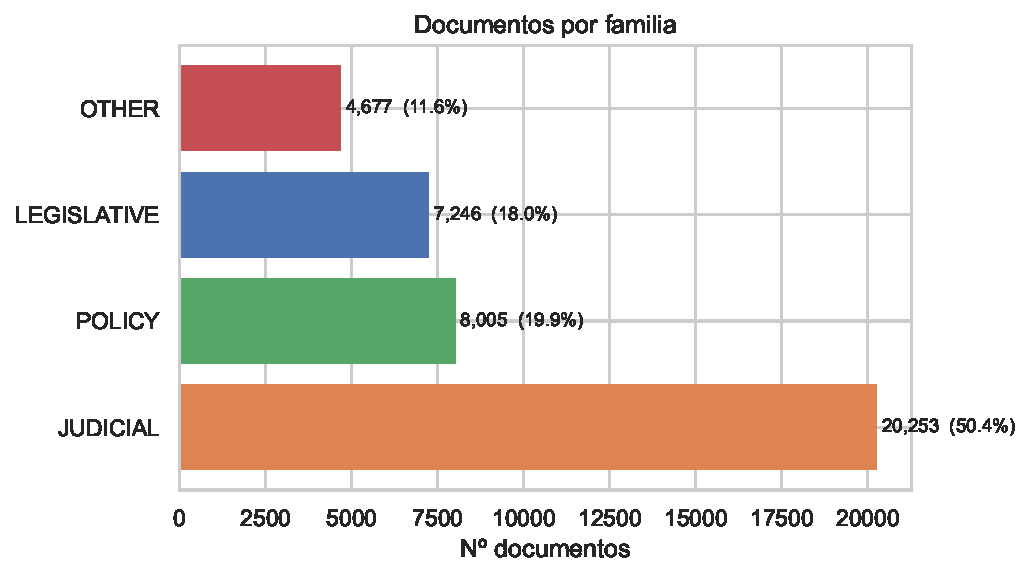
\includegraphics[width=\textwidth]{figures/eda_families}
  \caption{Distribución do corpus EUR-Lex por familia de documentos}
  \label{fig:corpus_familias}
  \fonte{elaboración propia a partir de datos de EUR-Lex}
\end{figure}

A heteroxeneidade de lonxitude entre familias é moi marcada
(Táboa~\ref{tab:lonxitude_familia} e Figura~\ref{fig:corpus_lonxitude}).
A familia JUDICIAL, maioritaria no corpus, contén documentos curtos
(mediana 336 palabras), cunha escisión natural entre avisos procesais
(11.517 documentos, mediana 264 palabras) e xurisprudencia substantiva
(8.736 documentos, mediana 631 palabras). A familia POLICY, pola contra,
presenta os documentos máis extensos (mediana 6.132 palabras; percentil~90
de 56.880 palabras). Esta variabilidade, de tres ordes de magnitude entre
familias, condiciona directamente as estratexias de segmentación avaliadas
no Experimento~2.

\begin{table}[H]
  \centering
  \caption{Percentís de lonxitude por familia de documentos (palabras)}
  \label{tab:lonxitude_familia}
  \rowcolors{2}{gray!10}{white}
  \begin{tabular}{lrrrr}
    \toprule
    \textbf{Familia} & \textbf{p25} & \textbf{p50 (mediana)}
      & \textbf{p75} & \textbf{p90} \\
    \midrule
    JUDICIAL    &   245 &    336 &    606 &  5.629 \\
    LEGISLATIVE &   353 &    938 &  4.945 & 18.369 \\
    OTHER       &   377 &  1.588 &  8.050 & 24.733 \\
    POLICY      & 1.904 &  6.132 & 20.892 & 56.880 \\
    \bottomrule
  \end{tabular}

  \smallskip
  {\footnotesize
    Mediana exacta (reconto de palabras); p25, p75 e p90 calculados
    como caracteres\,÷\,5 (aproximación).}
  \fonte{elaboración propia a partir de datos de EUR-Lex}
\end{table}

\begin{figure}[H]
  \centering
  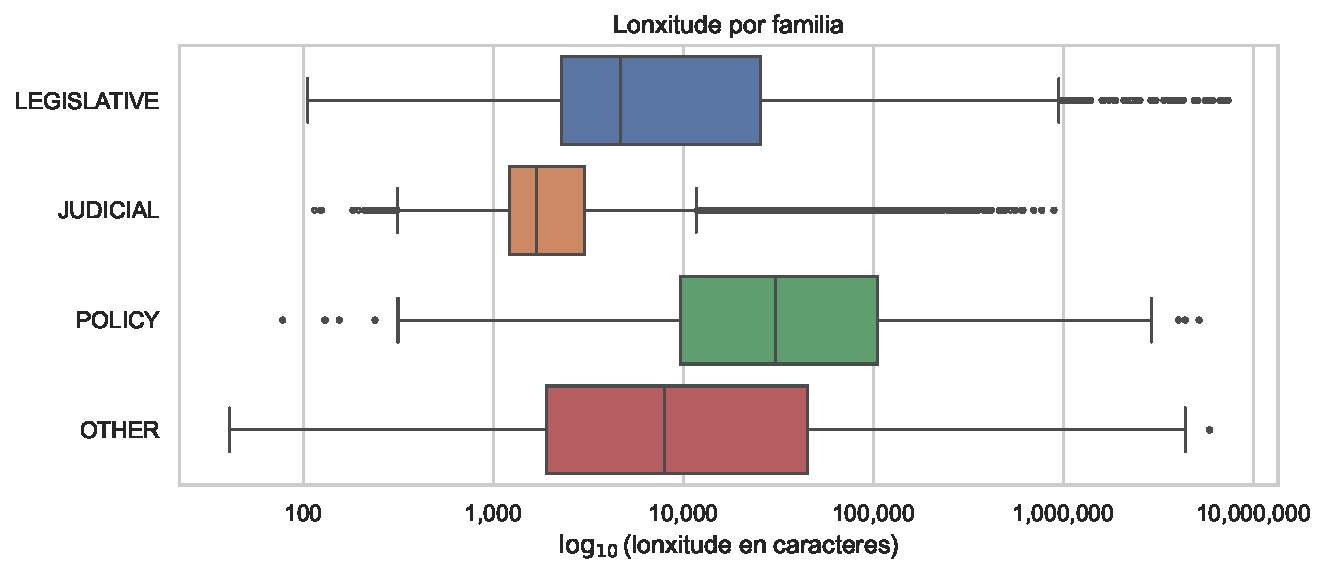
\includegraphics[width=\textwidth]{figures/eda_length_by_family}
  \caption{Distribución da lonxitude dos documentos por familia (escala logarítmica)}
  \label{fig:corpus_lonxitude}
  \fonte{elaboración propia a partir de datos de EUR-Lex}
\end{figure}

\subsection{Preprocesamento e limpeza}
\label{sec:preprocesamento}

Os documentos obtivéronse en formato JSONL desde o repositorio público
\texttt{gplsi/alia\_intellectual\_property} \citep{espinosa2025alia}
(\texttt{eurlex-en-md.jsonl}). Cada rexistro contén o texto do documento en
formato Markdown (campo \texttt{content}) e un obxecto de metadatos estruturado
(campo \texttt{metadata}) cos campos \texttt{celex}, \texttt{form},
\texttt{title}, \texttt{date}, \texttt{author} e \texttt{pages}, presentes no
100\,\% dos documentos do corpus.

A pipeline de inxesta (implementada como pipeline Kedro \texttt{ingestion}; véxase a
Sección~\ref{sec:kedro}) aplica sobre o corpus de partida (\texttt{eurlex-en-md.jsonl})
a seguinte limpeza do texto:

\begin{enumerate}
  \item \textbf{\texttt{\_strip\_header}:} Elimina a táboa de cabeceira da
    publicación (liñas do tipo \texttt{|}, \texttt{\#}, \texttt{[},
    \texttt{*}, \texttt{-}, \texttt{!}) ata o primeiro contido textual real
    (máis de 15~caracteres).
  \item \textbf{\texttt{\_remove\_footnote\_anchors}:} Suprime referencias
    de nota ao pé do tipo \texttt{[(1)(\#ntr...)]} e similares.
  \item \textbf{\texttt{\_remove\_top\_link}:} Elimina a ligazón de navegación
    \texttt{[Top](\#document1)} e o separador \texttt{---} orfo que o
    precede.
  \item \textbf{\texttt{\_strip\_links}:} Imaxes \texttt{![alt](url)} → nada;
    ligazóns \texttt{[texto](url)} → só o texto.
  \item \textbf{\texttt{\_strip\_markup}:} Converte a texto plano: negritas
    \texttt{**...**}, cursivas \texttt{*...*}, código en liña e cabeceiras
    \texttt{\#}.
  \item \textbf{\texttt{\_flatten\_two\_col\_tables}:} Táboas de dúas columnas
    \texttt{| (n) | texto |} (considerandos, subapartados de artigos) → texto
    plano continuo.
  \item \textbf{\texttt{\_normalize\_whitespace}:} \texttt{\textbackslash{}xa0}
    → espazo; 3 ou máis liñas en branco → 2; separadores \texttt{---}
    consecutivos → un.
\end{enumerate}

O texto resultante conserva todo o contido normativo (artigos, considerandos,
anexos, títulos en maiúsculas) e descarta exclusivamente os artefactos de formato
introducidos polo sistema de publicación. A pipeline produce
\texttt{corpus\_clean.jsonl} cos 40.181 documentos do corpus fonte, listos para a
selección do corpus de traballo descrita na Sección~\ref{sec:corpus_traballo}.

Esta etapa de limpeza implementouse integramente coa biblioteca estándar de Python
(\texttt{re} e \texttt{json}), sen dependencias de procesamento de linguaxe natural.

\subsection{Selección do corpus de traballo}
\label{sec:corpus_traballo}

O corpus fonte de 40.181 documentos abrangue todo o ámbito da propiedade intelectual,
un espazo demasiado amplo e heteroxéneo para construír un conxunto de avaliación coherente
con respostas verificables. Por iso, sobre o corpus xa limpo aplícase unha
\textbf{selección propia} (pipeline \texttt{corpus\_selection}) que illa un dominio
temático máis acoutado —o dereito de autor (\textit{copyright}) e dereitos afíns— co que
construír o golden dataset e executar todos os experimentos. Un documento incorpórase ao
corpus de traballo se cumpre as tres condicións seguintes:

\begin{enumerate}
  \item O seu título contén algunha das palabras clave do dominio: \textit{copyright},
    \textit{related right}, \textit{neighbouring right}, \textit{computer program} ou
    \textit{software}.
  \item A súa forma documental pertence a unha lista de tipos relevantes (sentenzas,
    conclusións do Avogado Xeral, autos, directivas, decisións, regulamentos,
    comunicacións, propostas e ditames, entre outras).
  \item A súa lonxitude supera un limiar mínimo, para descartar documentos demasiado
    curtos para soster preguntas substantivas.
\end{enumerate}

O resultado é un corpus de traballo de \textbf{363 documentos} (artefacto
\texttt{corpus\_copyright}). A súa composición por familia (Táboa~\ref{tab:corpus_traballo})
está aínda máis dominada pola xurisprudencia que o corpus fonte: a familia JUDICIAL
representa o 70,5\,\% dos documentos, fronte ao 50,4\,\% no corpus completo, o que reflicte
o peso da litixiosidade en materia de dereito de autor. Todos os resultados presentados na
Sección~\ref{sec:resultados} obtéñense sobre este corpus de traballo.

\begin{table}[H]
  \centering
  \caption{Composición do corpus de traballo (subconxunto de copyright) por familia}
  \label{tab:corpus_traballo}
  \rowcolors{2}{gray!10}{white}
  \begin{tabular}{lrr}
    \toprule
    \textbf{Familia} & \textbf{N.º docs} & \textbf{\%} \\
    \midrule
    JUDICIAL    & 256 & 70,5 \\
    POLICY      &  62 & 17,1 \\
    LEGISLATIVE &  24 &  6,6 \\
    OTHER       &  21 &  5,8 \\
    \midrule
    \textbf{Total} & \textbf{363} & 100 \\
    \bottomrule
  \end{tabular}
  \fonte{elaboración propia a partir de datos de EUR-Lex}
\end{table}

\subsection{Construción do golden dataset de avaliación}
\label{sec:golden_dataset}

A avaliación cuantitativa de calquera sistema RAG require un conxunto de probas
con respostas de referencia verificables (\textit{golden dataset}) que habilite
métricas como \textit{context recall} ou \textit{faithfulness}. Dado o custo
prohibitivo de redactar manualmente centenares de pares pregunta--resposta sobre
textos xurídicos, o conxunto xérase de forma sintética e semi-automática co módulo
\texttt{TestsetGenerator} de RAGAS (v0.3.9) sobre o corpus de traballo de
363~documentos, seguindo catro etapas.

\paragraph{1. Mostraxe estratificada.} Para evitar a sobrerrepresentación dos
documentos de lonxitude media, selecciónanse 75~documentos mediante mostraxe
estratificada por lonxitude (10, 25, 25 e 15~documentos nos estratos de 300--1.000,
1.000--5.000, 5.000--20.000 e máis de 20.000~palabras, respectivamente). Os
documentos longos sobrerrepreséntanse deliberadamente (un 20\,\% da mostra fronte
ao 9\,\% do corpus) por seren os máis ricos para preguntas que esixen combinar
información. A selección dentro de cada estrato realízase cun xerador pseudoaleatorio
inicializado cunha semente fixa (\texttt{seed=42}), o que fai a mostraxe reproducible.

\paragraph{2. Construción do grafo de coñecemento.} RAGAS transforma os
75~documentos nun grafo de coñecemento: divídeos en fragmentos polos seus titulares,
e sobre cada fragmento un LLM extrae os temas e as entidades nomeadas (organismos,
referencias normativas, datas) e descarta os fragmentos de baixa calidade. A partir
do solapamento de entidades entre fragmentos constrúense as relacións do grafo, que
son as que posibilitan máis adiante as preguntas multi-salto.

\paragraph{3. Xeración de pares pregunta--resposta.} Sobre o grafo xéranse escenarios
e, a partir de cada un, un LLM produce un par (pregunta, resposta de referencia). A
distribución é do 50\,\% entre dous tipos: \textit{single-hop} (preguntas
respondibles desde un único fragmento) e \textit{multi-hop específico} (preguntas que
esixen combinar feitos de dous fragmentos relacionados por entidades comúns). Cada
pregunta condiciónase a unha de dúas \textit{personas} —un avogado de propiedade
intelectual e un analista de políticas— e a unha combinación de estilo (gramática
correcta, gramática pobre, con erros ortográficos ou estilo de busca web) e lonxitude
(curta, media ou longa), co fin de cubrir formulacións heteroxéneas semellantes ás
dun usuario real. A resposta de referencia xérase coa instrución explícita de ser
fiel exclusivamente ao contido dos fragmentos de orixe, o que a habilita como
\textit{ground truth}.

\paragraph{4. Filtrado e revisión.} Os pares cuxa xeración produciu campos baleiros
descártanse automaticamente; sobre o resto realízase unha revisión manual de
coherencia para eliminar preguntas mal formadas ou ambiguas, sen reanotar as
respostas. O resultado final é un conxunto de \textbf{149~pares} pregunta--resposta
(75 \textit{single-hop} e 74 \textit{multi-hop}), cada un coa súa resposta de
referencia e os fragmentos de contexto que a sustentan.

A xeración realízase co LLM \texttt{deepseek-v4-flash} (temperatura~0) e os embeddings
do grafo de coñecemento co modelo \texttt{gemini-embedding-2}. Unha vez xerado, o
golden dataset permanece fixo en todos os experimentos para garantir comparacións
homoxéneas.

%% ============================================================
%%  3. METODOLOXÍA EXPERIMENTAL
%% ============================================================
\section{Metodoloxía experimental}
\label{sec:metodoloxia}

\subsection{Preguntas de investigación}
\label{sec:rqs}

Este traballo está guiado por cinco preguntas de investigación que se corresponden
coa secuencia dos experimentos realizados:

\begin{description}
  \item[\textbf{RQ1}:] Cal é o modelo de embedding que mellor representa o corpus
    xurídico EUR-Lex en termos de \textit{context recall} e \textit{context precision}?
  \item[\textbf{RQ2}:] Que estratexia de segmentación de documentos produce os chunks
    que mellor conservan o contexto relevante para as consultas do golden dataset?
  \item[\textbf{RQ3}:] A recuperación híbrida (BM25 + vectorial), a diversificación
    \ac{MMR} e a variación do número de documentos recuperados ($k$) melloran de forma
    consistente a recuperación densa estándar neste dominio?
  \item[\textbf{RQ4}:] As técnicas que actúan sobre a consulta (reescrita, HyDE,
    multi-query, RAG-Fusion, step-back, descomposición, self-query) ou engaden un paso
    de reordenación pos-recuperación (\textit{reranking} con cross-encoder ou LLM
    listwise) producen melloras relevantes sobre o mellor RAG base acumulado?
  \item[\textbf{RQ5}:] A pipeline RAG construída empiricamente mediante a ablación
    secuencial supera en calidade a un \textit{stack} que combina directamente técnicas
    consideradas estado da arte na literatura?
\end{description}

\subsection{Deseño experimental}
\label{sec:deseno_experimental}

O deseño experimental segue un enfoque de \textit{ablación secuencial} en cinco fases
de optimización (embedding, chunking, retrieval, expansión de consultas e reranking),
precedidas por unha liña base e seguidas dunha fase final de validación contra un
\textit{stack} estado da arte. En cada fase optimízase un compoñente da pipeline mentres
o resto permanece fixo; a mellor configuración de cada fase convértese en constante para
as fases seguintes.
Este deseño garante que as comparacións dentro de cada experimento son válidas (varía
só un compoñente á vez) e que o sistema RAG final está construído sobre as mellores
eleccións en cada capa.

Esta estratexia constitúe unha optimización \textit{greedy} (avara) e non garante un
óptimo global: a configuración escollida en cada fase é a mellor condicionada ás
decisións xa tomadas nas fases anteriores, pero poderían existir interaccións entre
compoñentes —por exemplo, entre o modelo de embedding e a estratexia de chunking— que
fixesen que outra combinación, non explorada, superase a obtida secuencialmente. Esta
limitación é análoga á da optimización secuencial de hiperparámetros, unha práctica
estándar cando o espazo combinatorio completo (o produto cartesiano de todas as
configuracións posibles en cada fase) resulta computacionalmente inabordable, e asume
implicitamente que os efectos principais de cada compoñente predominan sobre as súas
interaccións.

A secuencia de decisión é a seguinte:

\begin{enumerate}
  \item \textbf{Experimento~0 (Baseline):} establece a referencia mínima honesta contra
    a que se miden todas as melloras.
  \item \textbf{Experimento~1 (Embeddings):} fixa o mellor modelo de embedding para
    a recuperación en EUR-Lex.
  \item \textbf{Experimento~2 (Chunking):} fixa a mellor estratexia de segmentación
    co embedding xa fixado.
  \item \textbf{Experimento~3 (Retrieval):} fixa a mellor técnica de recuperación e o
    valor de $k$, co embedding e o chunking xa fixados.
  \item \textbf{Experimento~4 (Expansión de consultas):} avalía sobre o mellor RAG base
    acumulado as técnicas que actúan sobre a consulta antes da recuperación.
  \item \textbf{Experimento~5 (Reranking):} avalía a reordenación pos-recuperación dos
    candidatos sobre o mellor RAG base acumulado.
  \item \textbf{Experimento SOTA (Validación):} compara a pipeline óptima obtida
    empiricamente cun \textit{stack} que combina técnicas estado da arte da literatura,
    para situar o resultado nun marco de referencia externo.
\end{enumerate}

As \textbf{variables independentes} son as configuracións específicas de cada
experimento.
As \textbf{variables dependentes} son as seis métricas definidas na
Sección~\ref{sec:metricas}.
As \textbf{variables controladas} son o modelo LLM xerador, o corpus documental e o
golden dataset (construído na Sección~\ref{sec:golden_dataset}), que permanecen
constantes en todos os experimentos.
O número de documentos recuperados fíxa\-se en $\text{top}\_k = 5$ salvo nas
configuracións dos Experimentos~3 e 5, nos que se estuda explicitamente o efecto de $k$.

\subsection{Arquitectura do sistema experimental}
\label{sec:arquitectura}

Toda a experimentación execútase sobre unha infraestrutura modular implementada con Kedro
(Sección~\ref{sec:kedro}), organizada en cinco pipelines independentes que se encadean
nun fluxo de datos único (Figura~\ref{fig:arquitectura}). Os tres primeiros
—\texttt{ingestion}, \texttt{corpus\_selection} e \texttt{gold\_dataset}— prepáranse unha
soa vez e permanecen constantes en todos os experimentos, garantindo que o corpus de
traballo e o golden dataset son idénticos en todas as comparacións. Os pipelines
\texttt{rag\_base} (segmentación e indexación) e \texttt{evaluation} (execución da
recuperación e a xeración e cálculo das seis métricas RAGAS) conforman o ciclo RAG, cuxa
configuración se determina integramente por un ficheiro de parámetros
(\texttt{parameters\_exp*.yml}), un por cada experimento da ablación. Esta separación entre
a lóxica e a configuración é a que permite que cada fase da ablación se reduza a cambiar
parámetros, sen modificar código, e a que sustenta a reproducibilidade e a transferibilidade
do marco a outros dominios.

\begin{figure}[H]
  \centering
  \begin{tikzpicture}[
    font=\footnotesize,
    pipe/.style={rounded corners, draw=blue!55, fill=blue!8, line width=0.6pt,
                 text width=8.2cm, align=center, minimum height=8mm, inner sep=4pt},
    data/.style={draw=gray!60, fill=gray!10, line width=0.5pt,
                 text width=8.2cm, align=center, minimum height=6mm, inner sep=3pt},
    param/.style={rounded corners, draw=orange!75!black, fill=orange!15, line width=0.6pt,
                  text width=3.0cm, align=center, minimum height=10mm, inner sep=3pt},
    arr/.style={-{Latex[length=2.2mm]}, line width=0.6pt}
  ]
    \node[data] (src) {Fonte: EUR-Lex \texttt{(gplsi/alia\_intellectual\_property)}};
    \node[pipe, below=6mm of src] (ing) {\textbf{ingestion}\\[1pt] limpeza e preprocesamento $\rightarrow$ \texttt{corpus\_clean} (40.181 docs)};
    \node[pipe, below=6mm of ing] (sel) {\textbf{corpus\_selection}\\[1pt] selección do corpus de traballo (copyright) $\rightarrow$ \texttt{corpus\_copyright} (363 docs)};
    \node[pipe, below=6mm of sel] (gold) {\textbf{gold\_dataset}\\[1pt] xeración do golden dataset (149 pares pregunta--resposta)};
    \node[pipe, below=6mm of gold] (rag) {\textbf{rag\_base}\\[1pt] segmentación (chunking) e indexación vectorial $\rightarrow$ índice};
    \node[pipe, below=6mm of rag] (eval) {\textbf{evaluation}\\[1pt] execución RAG (retrieval + xeración) e avaliación RAGAS $\rightarrow$ seis métricas};

    \draw[arr] (src) -- (ing);
    \draw[arr] (ing) -- (sel);
    \draw[arr] (sel) -- (gold);
    \draw[arr] (gold) -- (rag);
    \draw[arr] (rag) -- (eval);

    \node[param, left=10mm of rag] (par) {\texttt{parameters\_exp*.yml}\\[1pt] (un por experimento)};
    \draw[arr] (par) -- (rag);

    \draw[arr, dashed] (eval.west) to[out=180, in=180]
      node[left, align=center, midway] {ablación\\secuencial} (par.west);
  \end{tikzpicture}
  \caption{Arquitectura do sistema experimental: pipelines Kedro e fluxo de datos}
  \label{fig:arquitectura}
  \fonte{elaboración propia}
\end{figure}

A Táboa~\ref{tab:pipelines} resume a responsabilidade de cada pipeline e os artefactos
que consome e produce, o que evidencia a modularidade do marco: cada etapa ten unha
entrada e unha saída ben definidas e pode reexecutarse de forma illada.

\begin{table}[H]
  \centering
  \caption{Pipelines Kedro: responsabilidade e artefactos de entrada e saída}
  \label{tab:pipelines}
  \footnotesize
  \rowcolors{2}{gray!10}{white}
  \begin{tabular}{>{\raggedright\arraybackslash}p{2.6cm}>{\raggedright\arraybackslash}p{6.0cm}>{\raggedright\arraybackslash}p{4.4cm}}
    \toprule
    \textbf{Pipeline} & \textbf{Responsabilidade} & \textbf{Entrada $\rightarrow$ Saída} \\
    \midrule
    \texttt{ingestion} & Limpeza e preprocesamento do texto en bruto &
      \texttt{raw\_corpus} $\rightarrow$ \texttt{corpus\_clean} (40.181) \\
    \texttt{corpus\_selection} & Selección do corpus de traballo (dominio de copyright) &
      \texttt{corpus\_clean} $\rightarrow$ \texttt{corpus\_copyright} (363) \\
    \texttt{gold\_dataset} & Mostraxe, grafo de coñecemento e xeración de pares pregunta--resposta &
      \texttt{corpus\_copyright} $\rightarrow$ \texttt{gold\_dataset} (149) \\
    \texttt{rag\_base} & Segmentación (chunking) e indexación vectorial &
      \texttt{corpus\_copyright} + parámetros $\rightarrow$ índice \\
    \texttt{evaluation} & Execución RAG (recuperación + xeración) e avaliación RAGAS &
      índice + \texttt{gold\_dataset} + parámetros $\rightarrow$ métricas \\
    \bottomrule
  \end{tabular}
  \fonte{elaboración propia}
\end{table}

\subsection{Técnicas avaliadas}
\label{sec:tecnicas_avaliadas}

\subsubsection{Experimento~0: Liña base (Naive RAG)}
\label{sec:exp0_baseline}

O obxectivo do Experimento~0 é establecer un punto de referencia honesto: un sistema
RAG mínimo cuxos scores documentan o punto de partida contra o que se miden todas as
melloras posteriores. A configuración é:

\begin{itemize}
  \item Corpus sen procesamento adicional máis alá da limpeza básica descrita na
    Sección~\ref{sec:preprocesamento}.
  \item Chunking de tamaño fixo: 256~tokens (segundo o tokenizador do propio modelo
    de embedding), solapamento de 25~tokens (arredor dun 10\,\%).
  \item Modelo de embedding: \texttt{BAAI/bge-base-en-v1.5} \citep{xiao2023c}
    (86~M de parámetros, 768 dimensións, xanela de contexto de 512~tokens).
  \item Retriever: busca por similitude coseno, $\text{top}\_k = 5$.
  \item Mesmo modelo LLM xerador para todos os experimentos.
\end{itemize}

Os scores obtidos gárdanse como \texttt{baseline\_v0} e constitúen a referencia
absoluta de comparación contra a que se mide cada mellora posterior.

\subsubsection{Experimento~1: Comparativa de modelos de embedding}
\label{sec:exp1_embeddings}

\textbf{Obxectivo:} identificar o modelo de embedding que mellor representa o corpus
EUR-Lex e recupera os chunks máis relevantes para as consultas do golden dataset.

\textbf{Variables fixas:} corpus, chunking (tamaño fixo, 256~tokens, solapamento de
25~tokens), retriever cosine, $\text{top}\_k = 5$, LLM, golden dataset.

\textbf{Variable independente:} modelo de embedding. Tómase como referencia o modelo
do Experimento~0 (\texttt{BAAI/bge-base-en-v1.5}, \citealt{xiao2023c}) e compárase
fronte a tres alternativas:

\begin{itemize}
  \item \texttt{BAAI/bge-m3} \citep{chen2024m3embedding}: modelo multilingüe da
    mesma familia BGE que xera simultaneamente representacións densas, esparsas
    e multi-vector, cunha xanela de contexto de até 8.192~tokens.
  \item \texttt{Qwen/Qwen3-Embedding-8B} \citep{zhang2025qwen3embedding}: modelo de
    embedding de 8.000~M de parámetros baseado na familia de LLM Qwen3, accedido
    mediante unha API de inferencia externa (Scaleway).
  \item \texttt{Snowflake/snowflake-arctic-embed-l-v2.0} \citep{yu2024arcticembed}:
    modelo multilingüe optimizado para tarefas de recuperación, baseado en
    XLM-RoBERTa-large (568~M de parámetros).
\end{itemize}

\textbf{Métricas de decisión:} Context Recall e Context Precision, xa que o embedding
afecta principalmente ao retriever. As demais métricas anótanse como observación para
detectar patróns inesperados (por exemplo, un cambio de embedding que mellore Context
Recall pero empeore Faithfulness indica un problema a investigar).

\subsubsection{Experimento~2: Comparativa de estratexias de chunking}
\label{sec:exp2_chunking}

\textbf{Obxectivo:} identificar a estratexia de segmentación que mellor conserva o
contexto relevante e encaixa coa estrutura formal dos documentos EUR-Lex.

\textbf{Variables fixas:} mellor embedding do Experimento~1, retriever cosine,
$\text{top}\_k = 5$, LLM, golden dataset. O tamaño de referencia pásase a
512~tokens, medidos co tokenizador do embedding gañador, con solapamento de
50~tokens onde a estratexia o permite.

\textbf{Variable independente:} estratexia de chunking. Avalíanse cinco estratexias:

\begin{itemize}
  \item \textbf{Tamaño fixo (\texttt{fixed\_size}).} \texttt{RecursiveCharacterTextSplitter}
    sobre o tokenizador do embedding gañador, con chunks de 512~tokens e
    solapamento de 50~tokens.
  \item \textbf{Por oracións (\texttt{sentence}).} Segmenta o texto en oracións
    e acumúlaas secuencialmente até acadar os 512~tokens, sen solapamento entre
    chunks consecutivos.
  \item \textbf{Estrutural (\texttt{structural}).} Segmenta seguindo a estrutura
    formal do documento: por artigos (identificados polo marcador \enquote{Article}
    seguido do número) nos actos lexislativos
    (regulamentos, directivas, decisións, etc.) e por parágrafos numerados nas
    resolucións xudiciais (sentenzas, conclusións, autos); as unidades resultantes
    que superan os 512~tokens subdivídense de forma recursiva, e os documentos sen
    marcadores estruturais recoñecibles segméntanse por parágrafos en branco.
  \item \textbf{Estrutural pai-fillo (\texttt{structural\_pc}).} Igual á estratexia
    anterior, pero cada chunk (\textit{fillo}, usado para indexar e recuperar)
    almacena tamén un \textit{contexto pai} —a unión das unidades estruturais
    adxacentes até 1.024~tokens— que se entrega ao LLM xerador en lugar do chunk
    orixinal (Sección~\ref{sec:parent_retriever_teoria}).
  \item \textbf{Semántico (\texttt{semantic}).} \texttt{SemanticChunker}
    \citep{kamradt2023semantic}: un modelo de embedding lixeiro local
    (\texttt{all-MiniLM-L6-v2}, \citealt{reimers2019sentence}) detecta puntos de
    ruptura semántica por percentil de disimilitude entre oracións consecutivas;
    os segmentos resultantes que superan os 512~tokens subdivídense de forma
    recursiva.
\end{itemize}

\textbf{Métricas de decisión:} Context Recall (¿o chunk recuperado contén a resposta?)
e Context Precision (¿os chunks recuperados son limpos e relevantes?).

\subsubsection{Experimento~3: Comparativa de técnicas de retrieval}
\label{sec:exp3_retrieval}

\textbf{Obxectivo:} avaliar que técnica de recuperación encontra mellor os chunks
relevantes, usando o embedding e o chunking xa fixados.

\textbf{Variables fixas:} mellor embedding do Experimento~1, mellor chunking do
Experimento~2, LLM, golden dataset.

\textbf{Variable independente:} técnica de retrieval e valor de $\text{top}\_k$.
As técnicas avalíanse en dous niveis:

\begin{itemize}
  \item \textbf{Nivel~1} (referencia):
    \begin{itemize}
      \item Busca por similitude coseno con $k \in \{3, 5, 10\}$ para illar o efecto
        do número de documentos recuperados.
    \end{itemize}
  \item \textbf{Nivel~2} (recuperación alternativa, con $k \in \{5, 10\}$):
    \begin{itemize}
      \item \ac{MMR} (diversidade nos chunks devoltos).
      \item BM25 \citep{robertson2009probabilistic} (recuperación esparsa pura).
      \item Busca híbrida BM25~+~vectorial con fusión por rango recíproco
        (\ac{RRF}, \citealt{cormack2009reciprocal}).
    \end{itemize}
\end{itemize}

\textbf{Métricas de decisión:} Context Recall, Context Precision e Noise Sensitivity.
Esta última introdúcese como criterio de decisión neste experimento por primeira vez,
xa que cuantifica directamente o impacto dos chunks irrelevantes sobre a xeración.

\subsubsection{Experimento~4: Expansión e transformación de consultas}
\label{sec:exp4_query_expansion}

\textbf{Obxectivo:} avaliar se as técnicas que transforman ou expanden a consulta antes
da recuperación producen melloras relevantes sobre o mellor RAG base acumulado.

\textbf{Variables fixas:} mellor configuración dos Experimentos~1--3, LLM, golden
dataset. Cada técnica avalíase de forma independente.

\begin{itemize}
  \item \textbf{HyDE:} o LLM xera un documento hipotético e este úsase como vector de
    busca \citep{gao2022precise}.
  \item \textbf{Multi-Query:} xéranse $n = 3$ variantes da consulta e fúndense os
    resultados (Sección~\ref{sec:query_rewriting_teoria}).
  \item \textbf{RAG-Fusion:} variantes da consulta combinadas mediante fusión por rango
    recíproco (\ac{RRF}).
  \item \textbf{Reescrita de consultas} (\textit{query rewriting},
    Sección~\ref{sec:query_rewriting_teoria}).
  \item \textbf{Step-Back:} o LLM xera unha pregunta máis xenérica para recuperar
    contexto de fondo.
  \item \textbf{Descomposición:} a consulta divídese en sub-preguntas que se recuperan
    de forma independente.
  \item \textbf{Self-Query:} extracción de filtros de metadatos a partir da consulta
    en linguaxe natural (Sección~\ref{sec:selfquery_teoria}).
\end{itemize}

\textbf{Métricas de decisión:} Context Recall, Context Precision e Noise Sensitivity.
As melloras de xeración (Faithfulness, Answer Relevancy) anótanse como evidencia
secundaria.

\subsubsection{Experimento~5: Reranking pos-recuperación}
\label{sec:exp5_reranking}

\textbf{Obxectivo:} avaliar se a reordenación dos candidatos recuperados mediante un
\textit{reranker} mellora a calidade do contexto e da resposta sobre o mellor RAG base
acumulado.

\textbf{Variables fixas:} mellor configuración dos Experimentos~1--3, LLM, golden
dataset.

\textbf{Variable independente:} tipo de reranker e valor de $\text{top}\_k$. Aplícase
unha cascada de dúas etapas: o retriever base recupera un \textit{pool} de candidatos
e un reranker reordénaos para reter os $\text{top}\_k \in \{5, 10\}$ finais. Avalíanse
dous tipos de reranker:

\begin{itemize}
  \item \textbf{Cross-encoder:} \texttt{BAAI/bge-reranker-v2-m3}
    \citep{chen2024m3embedding}, da mesma familia que o modelo de embedding
    \texttt{bge-m3}.
  \item \textbf{LLM listwise:} o propio LLM xerador recibe os candidatos nunha soa
    chamada e devolve a orde de relevancia.
\end{itemize}

\textbf{Métricas de decisión:} Context Recall, Context Precision, Noise Sensitivity e
Faithfulness, dado que o reranking afecta tanto á calidade do contexto como á da
xeración.

\subsubsection{Experimento SOTA: validación contra un \textit{stack} estado da arte}
\label{sec:expsota}

\textbf{Obxectivo:} situar a pipeline óptima obtida pola ablación secuencial nun marco
de referencia externo, comparándoa cun \textit{stack} maximalista que combina a técnica
máis avanzada \emph{sobre o papel} de cada dimensión —embedding \texttt{Qwen3-Embedding-8B}
(líder en MTEB), chunking semántico, recuperación híbrida BM25\,+\,vectorial con \ac{RRF},
expansión de consultas RAG-Fusion e reranking listwise por LLM—, en lugar de seleccionar
cada compoñente empiricamente fase a fase.

\textbf{Variables fixas:} LLM e golden dataset. \textbf{Comparación:} tres pipelines
—o baseline (Naive RAG, Experimento~0), o \textit{stack} SOTA da literatura e a pipeline
empírica óptima (resultado da ablación)— avalíanse coas seis métricas RAGAS.

\subsection{Métricas de avaliación}
\label{sec:metricas}

Empréganse seis métricas do framework RAGAS (definidas formalmente na
Sección~\ref{sec:ragas_teoria}). As métricas clasifícanse como \textbf{primarias}
(criterio de decisión no experimento correspondente) ou \textbf{secundarias}
(rexistradas como observación en todos os experimentos para detectar efectos
colaterais).

\begin{description}
  \item[Context Recall.] Métrica de recuperación. Mide en que medida o contexto
    recuperado contén toda a información necesaria para responder á pregunta.
    \textbf{Primaria} nos Experimentos~1--5.

  \item[Context Precision.] Métrica de recuperación. Mide se os chunks relevantes
    están posicionados nos rangos superiores do contexto recuperado.
    \textbf{Primaria} nos Experimentos~1--5.

  \item[Context Entity Recall.] Métrica de recuperación. Mide a proporción de entidades
    da resposta de referencia presentes no contexto recuperado.
    \textbf{Secundaria} en todos os experimentos.

  \item[Noise Sensitivity.] Métrica de recuperación. Mide a proporción de afirmacións
    incorrectas na resposta atribuíbles a chunks irrelevantes no contexto.
    \textbf{Primaria} nos Experimentos~3, 4 e 5.

  \item[Faithfulness.] Métrica de xeración. Mide en que medida as afirmacións da
    resposta están apoiadas polo contexto recuperado (Ecuación~\ref{eq:faithfulness}).
    \textbf{Primaria} no Experimento~5.

  \item[Response Relevancy.] Métrica de xeración. Mide se a resposta xerada aborda
    a pregunta do usuario (Ecuación~\ref{eq:answer_relevancy}).
    \textbf{Secundaria} en todos os experimentos.
\end{description}

Todas as métricas RAGAS están normalizadas no intervalo $[0, 1]$. Como criterio de
decisión agregado para as métricas de recuperación emprégase a suma
$\text{P{+}R} = \text{Context Precision} + \text{Context Recall}$, que resume nun único
valor a calidade global da recuperación de cada configuración.

A Táboa~\ref{tab:metricas_experimentos} resume o papel de cada métrica en cada
experimento.

\begin{table}[H]
  \centering
  \caption{Métricas de decisión~(P) e de observación~(S) por experimento}
  \label{tab:metricas_experimentos}
  \rowcolors{2}{gray!10}{white}
  \begin{tabular}{lcccccc}
    \toprule
    \textbf{Métrica}       & \textbf{Exp.~0} & \textbf{Exp.~1} & \textbf{Exp.~2}
                           & \textbf{Exp.~3} & \textbf{Exp.~4} & \textbf{Exp.~5} \\
    \midrule
    Context Recall         & S & P & P & P & P & P \\
    Context Precision      & S & P & P & P & P & P \\
    Context Entity Recall  & S & S & S & S & S & S \\
    Noise Sensitivity      & S & S & S & P & P & P \\
    Faithfulness           & S & S & S & S & S & P \\
    Response Relevancy     & S & S & S & S & S & S \\
    \bottomrule
  \end{tabular}

  \smallskip
  {\footnotesize
    P\,=\,métrica de decisión (criterio de elección da mellor configuración);
    S\,=\,métrica secundaria (rexistrada para observación).
  }
  \fonte{elaboración propia}
\end{table}


%% ============================================================
%%  RESULTADOS E DISCUSIÓN
%% ============================================================
\section{Resultados e discusión}
\label{sec:resultados}

Nesta sección preséntanse os resultados da ablación secuencial descrita na
Sección~\ref{sec:metodoloxia}, avaliada sobre o golden dataset de 149 pares
pregunta--resposta (75 \textit{single-hop} e 74 \textit{multi-hop}). Cada
configuración avalíase coas seis métricas RAGAS; como criterio agregado de decisión
para a recuperación emprégase $\text{P{+}R} = \text{Context Precision} +
\text{Context Recall}$. En todas as táboas, as columnas abreviadas son CR~(Context
Recall), CP~(Context Precision), CER~(Context Entity Recall), F~(Faithfulness),
RR~(Response Relevancy) e NS~(Noise Sensitivity); a fila gañadora de cada fase
destácase en \textbf{negra}.

\subsection{Experimento~1: modelos de embedding}
\label{sec:res_exp1}

A Táboa~\ref{tab:res_exp1} recolle a comparativa dos catro modelos de embedding sobre
a configuración base. O modelo \texttt{bge-m3} domina con claridade: eleva o P+R desde
0{,}756 (baseline \texttt{bge-base-en-v1.5}) até 0{,}999, unha mellora absoluta de
\textbf{+0{,}243}, a maior de toda a ablación. A mellora é transversal —Context Recall
pasa de 0{,}453 a 0{,}583 e Response Relevancy de 0{,}423 a 0{,}561— o que confirma que
a representación multilingüe e densa-esparsa-multivector de \texttt{bge-m3} captura
mellor a semántica do corpus xurídico que os modelos máis pequenos. O modelo
\texttt{qwen3-embedding-8b}, a pesar do seu tamaño (8.000~M de parámetros), queda por
detrás (P+R 0{,}889), o que indica que o tamaño do modelo non garante por si só unha
mellor recuperación neste dominio.

\begin{table}[H]
  \centering
  \caption{Resultados do Experimento~1 (modelos de embedding)}
  \label{tab:res_exp1}
  \footnotesize
  \rowcolors{2}{gray!10}{white}
  \begin{tabular}{lccccccc}
    \toprule
    \textbf{Configuración} & \textbf{CR} & \textbf{CP} & \textbf{CER} & \textbf{F}
                           & \textbf{RR} & \textbf{NS} & \textbf{P+R} \\
    \midrule
    bge-base-en-v1.5 (baseline) & 0,453 & 0,304 & 0,324 & 0,833 & 0,423 & 0,390 & 0,756 \\
    snowflake-arctic-embed-l    & 0,463 & 0,312 & 0,325 & 0,843 & 0,456 & 0,359 & 0,775 \\
    qwen3-embedding-8b          & 0,502 & 0,387 & 0,308 & 0,866 & 0,456 & 0,353 & 0,889 \\
    \textbf{bge-m3 (gañador)}   & \textbf{0,583} & \textbf{0,416} & \textbf{0,384} & \textbf{0,881} & \textbf{0,561} & \textbf{0,466} & \textbf{0,999} \\
    \bottomrule
  \end{tabular}
  \fonte{elaboración propia}
\end{table}

\begin{figure}[H]
  \centering
  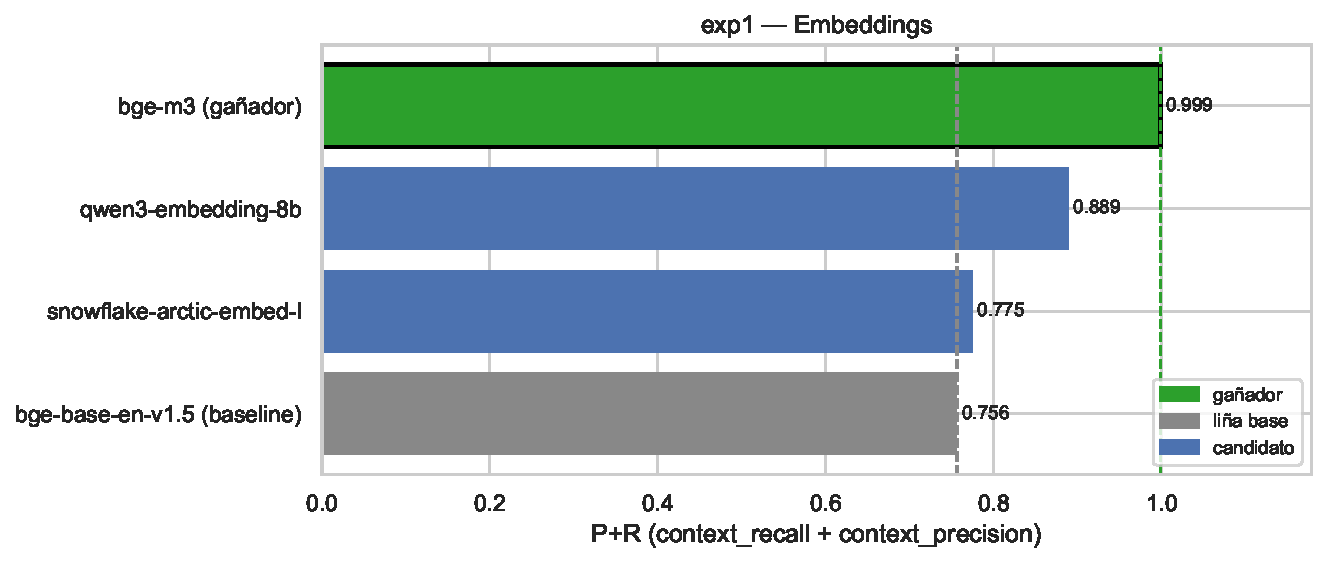
\includegraphics[width=\textwidth]{figures/exp1_embeddings}
  \caption{Comparativa de modelos de embedding (Experimento~1)}
  \label{fig:res_exp1}
  \fonte{elaboración propia}
\end{figure}

\subsection{Experimento~2: estratexias de chunking}
\label{sec:res_exp2}

Fixado \texttt{bge-m3}, avaliáronse cinco estratexias de segmentación fronte ao chunking
de tamaño fixo de 256~tokens da liña base (Táboa~\ref{tab:res_exp2}). O resultado é
contraintuitivo: \textbf{ningunha estratexia supera o chunking fixo de 256~tokens}
(P+R 0{,}999). A segmentación por oracións queda moi preto (0{,}993) e mellora o Context
Recall (0{,}615), pero a un custo en Context Precision. A segmentación estrutural —que a
priori encaixaría coa organización por artigos dos documentos EUR-Lex— resulta a peor
opción (P+R 0{,}729), probablemente porque xera unidades de tamaño moi heteroxéneo que
fragmentan o contexto relevante. En consecuencia, mantense o chunking fixo de 256~tokens.

\begin{table}[H]
  \centering
  \caption{Resultados do Experimento~2 (estratexias de chunking)}
  \label{tab:res_exp2}
  \footnotesize
  \rowcolors{2}{gray!10}{white}
  \begin{tabular}{lccccccc}
    \toprule
    \textbf{Configuración} & \textbf{CR} & \textbf{CP} & \textbf{CER} & \textbf{F}
                           & \textbf{RR} & \textbf{NS} & \textbf{P+R} \\
    \midrule
    \textbf{fixed 256 (gañador = baseline)} & \textbf{0,583} & \textbf{0,416} & \textbf{0,384} & \textbf{0,881} & \textbf{0,561} & \textbf{0,466} & \textbf{0,999} \\
    fixed 512            & 0,580 & 0,333 & 0,356 & 0,805 & 0,479 & 0,425 & 0,913 \\
    sentence             & 0,615 & 0,378 & 0,362 & 0,870 & 0,460 & 0,405 & 0,993 \\
    structural           & 0,447 & 0,281 & 0,324 & 0,891 & 0,460 & 0,384 & 0,729 \\
    structural + parent  & 0,590 & 0,368 & 0,348 & 0,849 & 0,438 & 0,420 & 0,958 \\
    semantic             & 0,594 & 0,297 & 0,346 & 0,866 & 0,462 & 0,471 & 0,891 \\
    \bottomrule
  \end{tabular}
  \fonte{elaboración propia}
\end{table}

\begin{figure}[H]
  \centering
  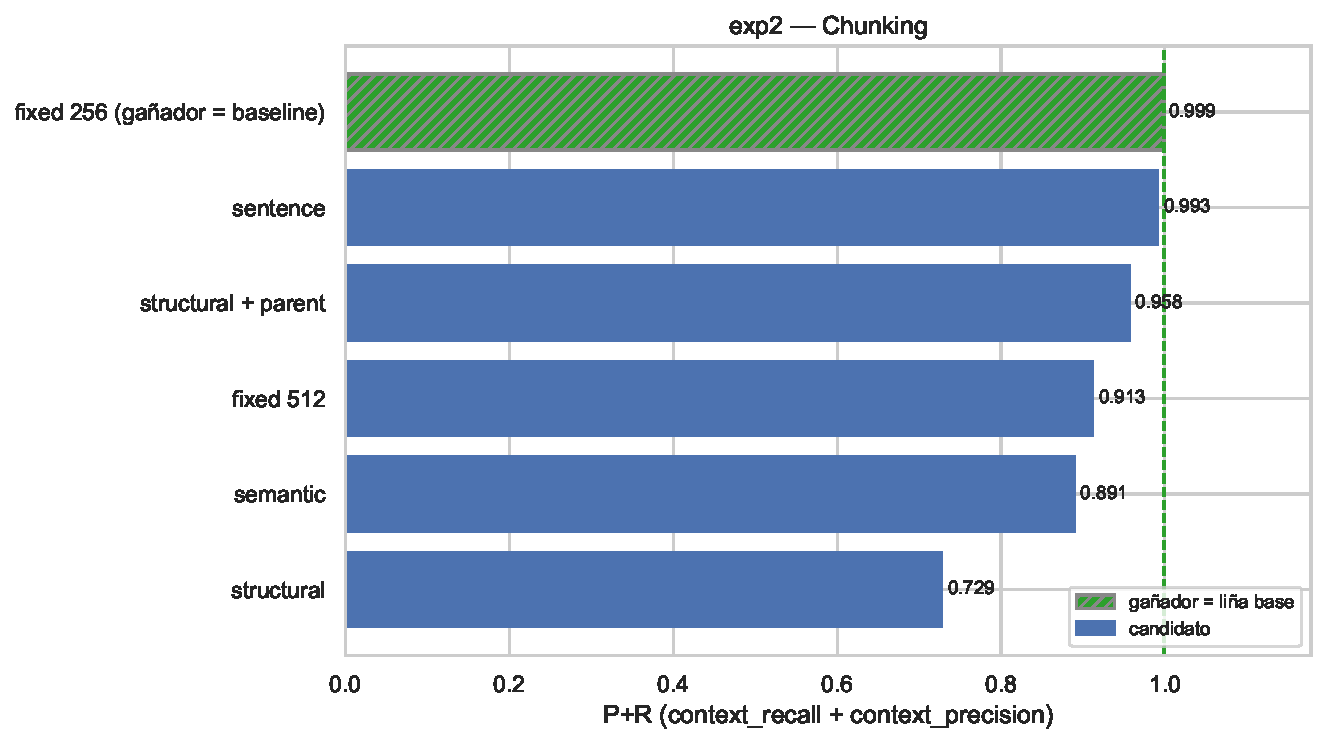
\includegraphics[width=\textwidth]{figures/exp2_chunking}
  \caption{Comparativa de estratexias de chunking (Experimento~2)}
  \label{fig:res_exp2}
  \fonte{elaboración propia}
\end{figure}

\subsection{Experimento~3: técnicas de retrieval}
\label{sec:res_exp3}

A Táboa~\ref{tab:res_exp3} compara as técnicas de recuperación. Dúas conclusións son
claras. Primeira, aumentar $k$ de 5 a 10 mellora a recuperación densa (de 0{,}999 a
1{,}050 en P+R). Segunda, a diversificación \ac{MMR} con $k = 10$ é a mellor opción
(\textbf{P+R 1{,}094}, Context Recall 0{,}711), ao recuperar contextos máis variados que
reducen a redundancia. As alternativas esparsa (BM25) e híbrida non superan a densa neste
dominio: aínda que BM25 acada un Context Recall alto (0{,}656), a súa Context Precision
cae drasticamente (0{,}258), o que penaliza o agregado. Adóptase, polo tanto, \texttt{mmr~k10}.

\begin{table}[H]
  \centering
  \caption{Resultados do Experimento~3 (técnicas de retrieval)}
  \label{tab:res_exp3}
  \footnotesize
  \rowcolors{2}{gray!10}{white}
  \begin{tabular}{lccccccc}
    \toprule
    \textbf{Configuración} & \textbf{CR} & \textbf{CP} & \textbf{CER} & \textbf{F}
                           & \textbf{RR} & \textbf{NS} & \textbf{P+R} \\
    \midrule
    cosine k5 (baseline) & 0,583 & 0,416 & 0,384 & 0,881 & 0,561 & 0,466 & 0,999 \\
    cosine k10           & 0,644 & 0,406 & 0,386 & 0,905 & 0,575 & 0,392 & 1,050 \\
    bm25 k10             & 0,656 & 0,258 & 0,384 & 0,826 & 0,403 & 0,409 & 0,914 \\
    hybrid k10           & 0,614 & 0,272 & 0,369 & 0,845 & 0,566 & 0,378 & 0,886 \\
    \textbf{mmr k10 (gañador)} & \textbf{0,711} & \textbf{0,383} & \textbf{0,377} & \textbf{0,899} & \textbf{0,590} & \textbf{0,429} & \textbf{1,094} \\
    \bottomrule
  \end{tabular}
  \fonte{elaboración propia}
\end{table}

\begin{figure}[H]
  \centering
  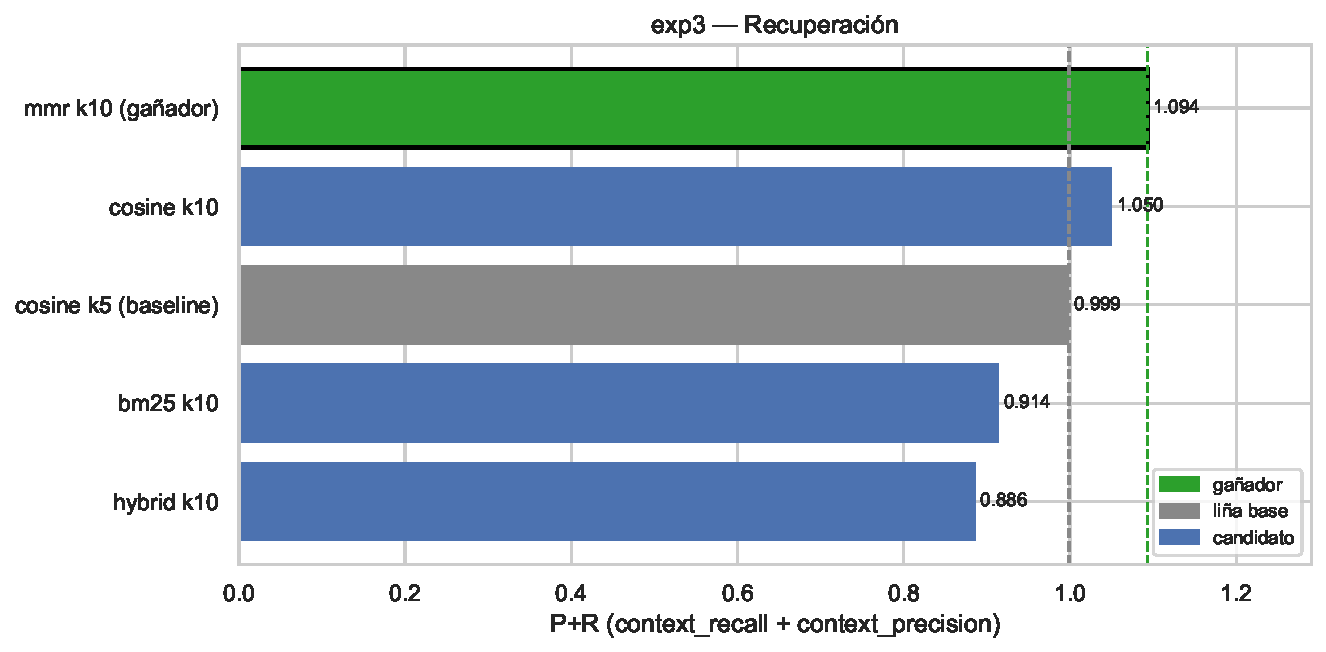
\includegraphics[width=\textwidth]{figures/exp3_retrieval}
  \caption{Comparativa de técnicas de retrieval (Experimento~3)}
  \label{fig:res_exp3}
  \fonte{elaboración propia}
\end{figure}

\subsection{Experimento~4: expansión e transformación de consultas}
\label{sec:res_exp4}

Sobre a base \texttt{mmr~k10} (P+R 1{,}094) avaliáronse sete técnicas de transformación
da consulta (Táboa~\ref{tab:res_exp4}). O resultado é negativo: \textbf{ningunha técnica
supera a base sen expansión}. A mellor, Multi-Query, queda lixeiramente por debaixo
(1{,}047), e técnicas como HyDE (0{,}846) ou Self-Query (0{,}823) deterioran
notablemente a recuperación. A interpretación é que, nun corpus xurídico onde as
consultas xa son específicas e están ben formuladas, a expansión introduce ruído que
desvía a recuperación máis do que a axuda. En consecuencia, a pipeline non incorpora
ningunha técnica de expansión de consultas.

\begin{table}[H]
  \centering
  \caption{Resultados do Experimento~4 (expansión de consultas)}
  \label{tab:res_exp4}
  \footnotesize
  \rowcolors{2}{gray!10}{white}
  \begin{tabular}{lccccccc}
    \toprule
    \textbf{Configuración} & \textbf{CR} & \textbf{CP} & \textbf{CER} & \textbf{F}
                           & \textbf{RR} & \textbf{NS} & \textbf{P+R} \\
    \midrule
    \textbf{mmr k10 (sen expansión)} & \textbf{0,711} & \textbf{0,383} & \textbf{0,377} & \textbf{0,899} & \textbf{0,590} & \textbf{0,429} & \textbf{1,094} \\
    Multi-Query   & 0,665 & 0,382 & 0,389 & 0,878 & 0,582 & 0,422 & 1,047 \\
    RAG-Fusion    & 0,650 & 0,365 & 0,359 & 0,918 & 0,515 & 0,387 & 1,015 \\
    Step-Back     & 0,654 & 0,349 & 0,341 & 0,895 & 0,544 & 0,339 & 1,003 \\
    Rewrite       & 0,633 & 0,354 & 0,354 & 0,938 & 0,568 & 0,408 & 0,987 \\
    Decomposition & 0,660 & 0,283 & 0,383 & 0,919 & 0,593 & 0,420 & 0,942 \\
    HyDE          & 0,598 & 0,247 & 0,336 & 0,877 & 0,559 & 0,397 & 0,846 \\
    Self-Query    & 0,485 & 0,338 & 0,236 & 0,810 & 0,438 & 0,354 & 0,823 \\
    \bottomrule
  \end{tabular}
  \fonte{elaboración propia}
\end{table}

\begin{figure}[H]
  \centering
  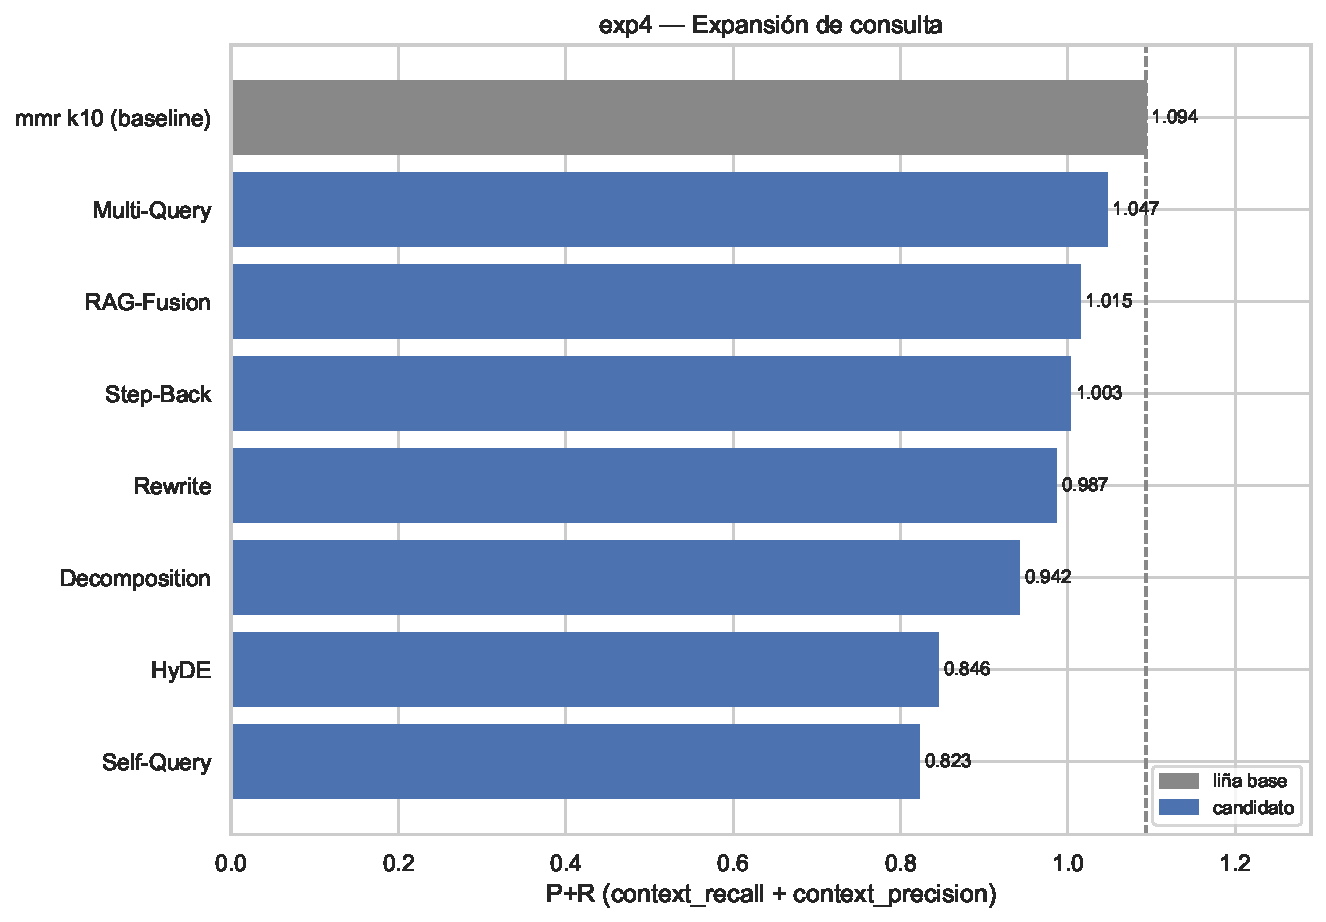
\includegraphics[width=\textwidth]{figures/exp4_query_expansion}
  \caption{Comparativa de técnicas de expansión de consultas (Experimento~4)}
  \label{fig:res_exp4}
  \fonte{elaboración propia}
\end{figure}

\subsection{Experimento~5: reranking pos-recuperación}
\label{sec:res_exp5}

A reordenación pos-recuperación é a segunda mellora máis importante da ablación
(Táboa~\ref{tab:res_exp5}). O cross-encoder \texttt{bge-reranker-v2-m3} con $k = 10$
acada o mellor resultado global do estudo: \textbf{P+R 1{,}203} (\textbf{+0{,}109}
sobre a base \texttt{mmr~k10}), ademais do mellor Faithfulness (0{,}951) e a mellor
Response Relevancy (0{,}650) de toda a experimentación. Os dous tipos de reranker
melloran a base, pero o cross-encoder supera ao reranking listwise por LLM, cun custo
computacional moi inferior (unha pasada do modelo cross-encoder fronte a unha chamada
ao LLM xerador). Adóptase \texttt{cross-encoder~k10} como último compoñente da pipeline.

\begin{table}[H]
  \centering
  \caption{Resultados do Experimento~5 (reranking)}
  \label{tab:res_exp5}
  \footnotesize
  \rowcolors{2}{gray!10}{white}
  \begin{tabular}{lccccccc}
    \toprule
    \textbf{Configuración} & \textbf{CR} & \textbf{CP} & \textbf{CER} & \textbf{F}
                           & \textbf{RR} & \textbf{NS} & \textbf{P+R} \\
    \midrule
    mmr k10 (sen rerank)   & 0,711 & 0,383 & 0,377 & 0,899 & 0,590 & 0,429 & 1,094 \\
    cross-encoder k5       & 0,708 & 0,479 & 0,374 & 0,924 & 0,556 & 0,403 & 1,187 \\
    LLM listwise k5        & 0,666 & 0,488 & 0,381 & 0,901 & 0,573 & 0,381 & 1,154 \\
    LLM listwise k10       & 0,721 & 0,463 & 0,441 & 0,890 & 0,579 & 0,432 & 1,184 \\
    \textbf{cross-encoder k10 (gañador)} & \textbf{0,756} & \textbf{0,447} & \textbf{0,389} & \textbf{0,951} & \textbf{0,650} & \textbf{0,408} & \textbf{1,203} \\
    \bottomrule
  \end{tabular}
  \fonte{elaboración propia}
\end{table}

\begin{figure}[H]
  \centering
  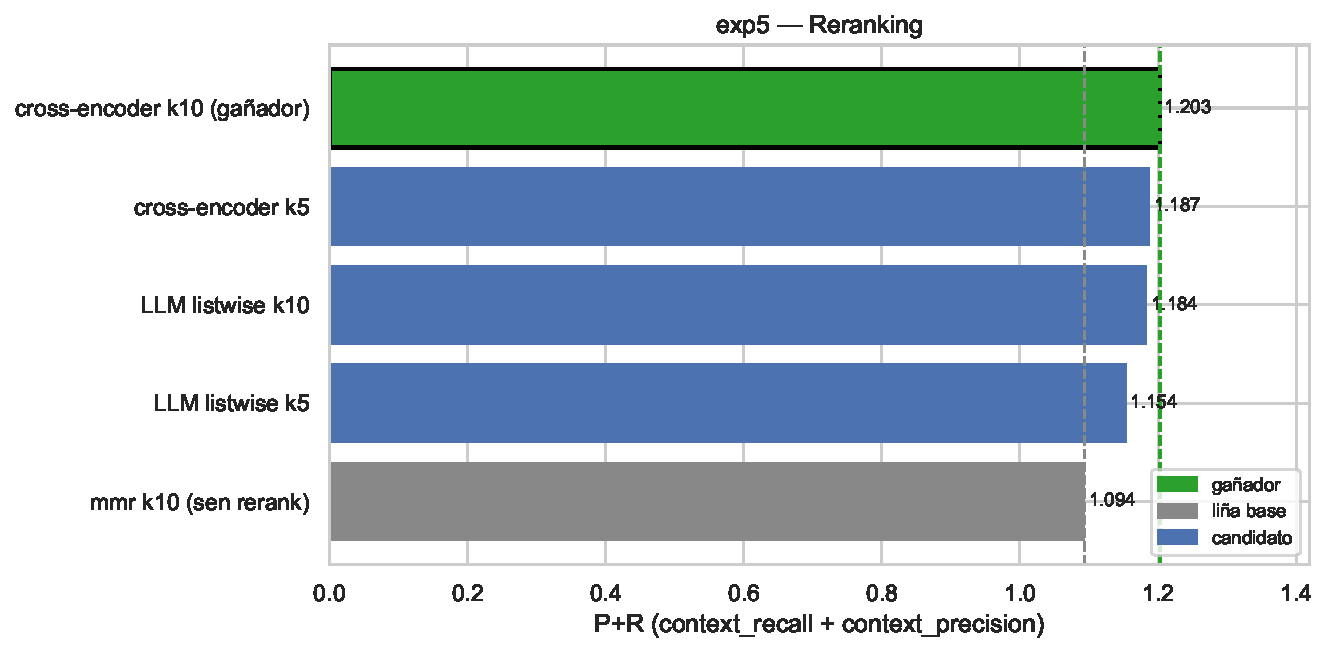
\includegraphics[width=\textwidth]{figures/exp5_reranking}
  \caption{Comparativa de técnicas de reranking (Experimento~5)}
  \label{fig:res_exp5}
  \fonte{elaboración propia}
\end{figure}

\subsection{Progresión global e pipeline final}
\label{sec:res_progresion}

A Táboa~\ref{tab:res_progresion} e a Figura~\ref{fig:res_progresion} resumen a progresión
acumulada da ablación. A pipeline final óptima componse de: embedding \texttt{bge-m3},
chunking fixo de 256~tokens, recuperación \texttt{mmr} con $k = 10$, sen expansión de
consultas, e reranking con cross-encoder \texttt{bge-reranker-v2-m3} ($k = 10$). Esta
configuración eleva o P+R desde 0{,}756 (baseline) até 1{,}203, unha mellora relativa do
\textbf{59\,\%}. As tres decisións con impacto foron, por orde de magnitude, o embedding
(+0{,}243), o reranking (+0{,}109) e o retrieval (+0{,}095); o chunking e a expansión de
consultas non achegaron melloras.

\begin{table}[H]
  \centering
  \caption{Progresión acumulada da ablación secuencial (métrica P+R)}
  \label{tab:res_progresion}
  \rowcolors{2}{gray!10}{white}
  \begin{tabular}{lcc}
    \toprule
    \textbf{Decisión acumulada} & \textbf{P+R} & \textbf{$\Delta$} \\
    \midrule
    Baseline (Exp.~0)            & 0,756 & --- \\
    + Embedding: bge-m3          & 0,999 & +0,243 \\
    + Chunking: fixed 256        & 0,999 & +0,000 \\
    + Retrieval: mmr k10         & 1,094 & +0,095 \\
    + Expansión de consultas: —  & 1,094 & +0,000 \\
    \textbf{+ Reranking: ce k10} & \textbf{1,203} & \textbf{+0,109} \\
    \bottomrule
  \end{tabular}
  \fonte{elaboración propia}
\end{table}

\begin{figure}[H]
  \centering
  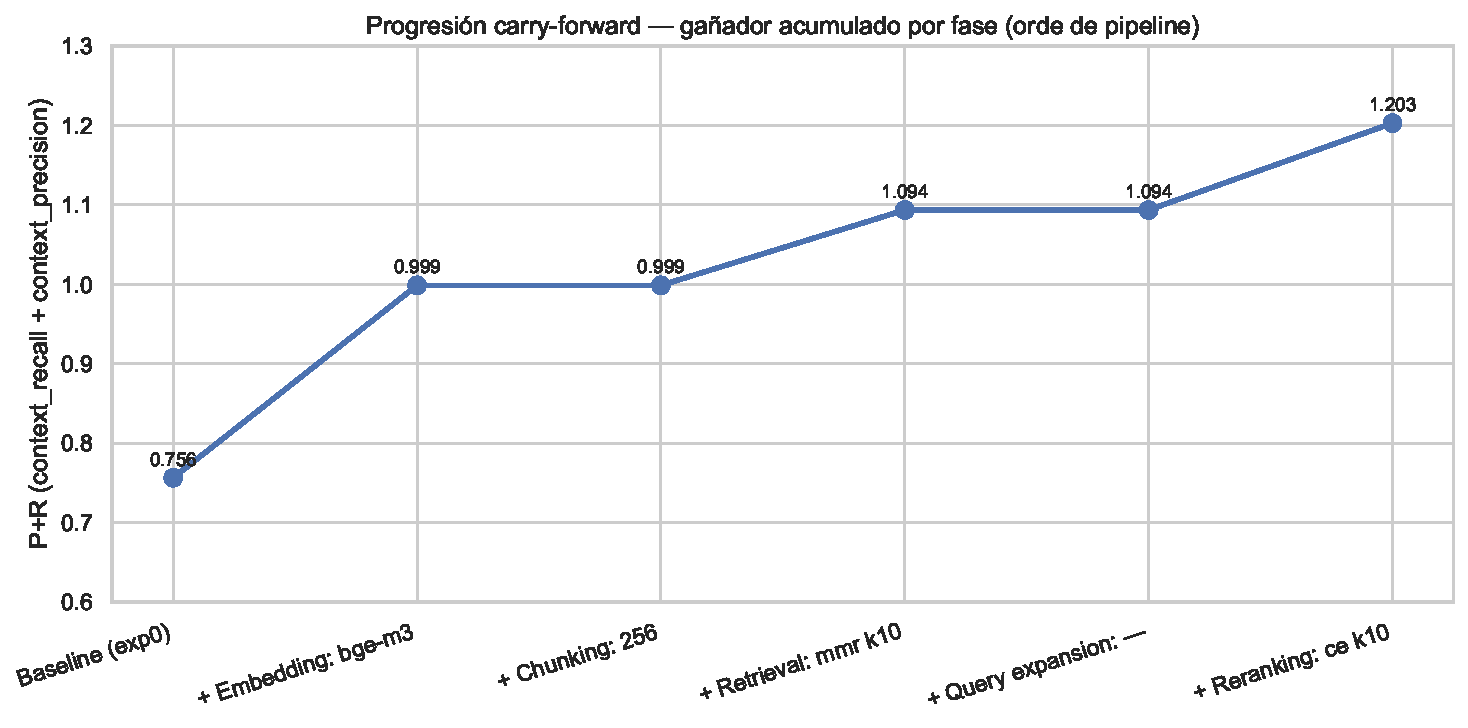
\includegraphics[width=\textwidth]{figures/progression}
  \caption{Progresión acumulada do P+R ao longo da ablación secuencial}
  \label{fig:res_progresion}
  \fonte{elaboración propia}
\end{figure}

\begin{figure}[H]
  \centering
  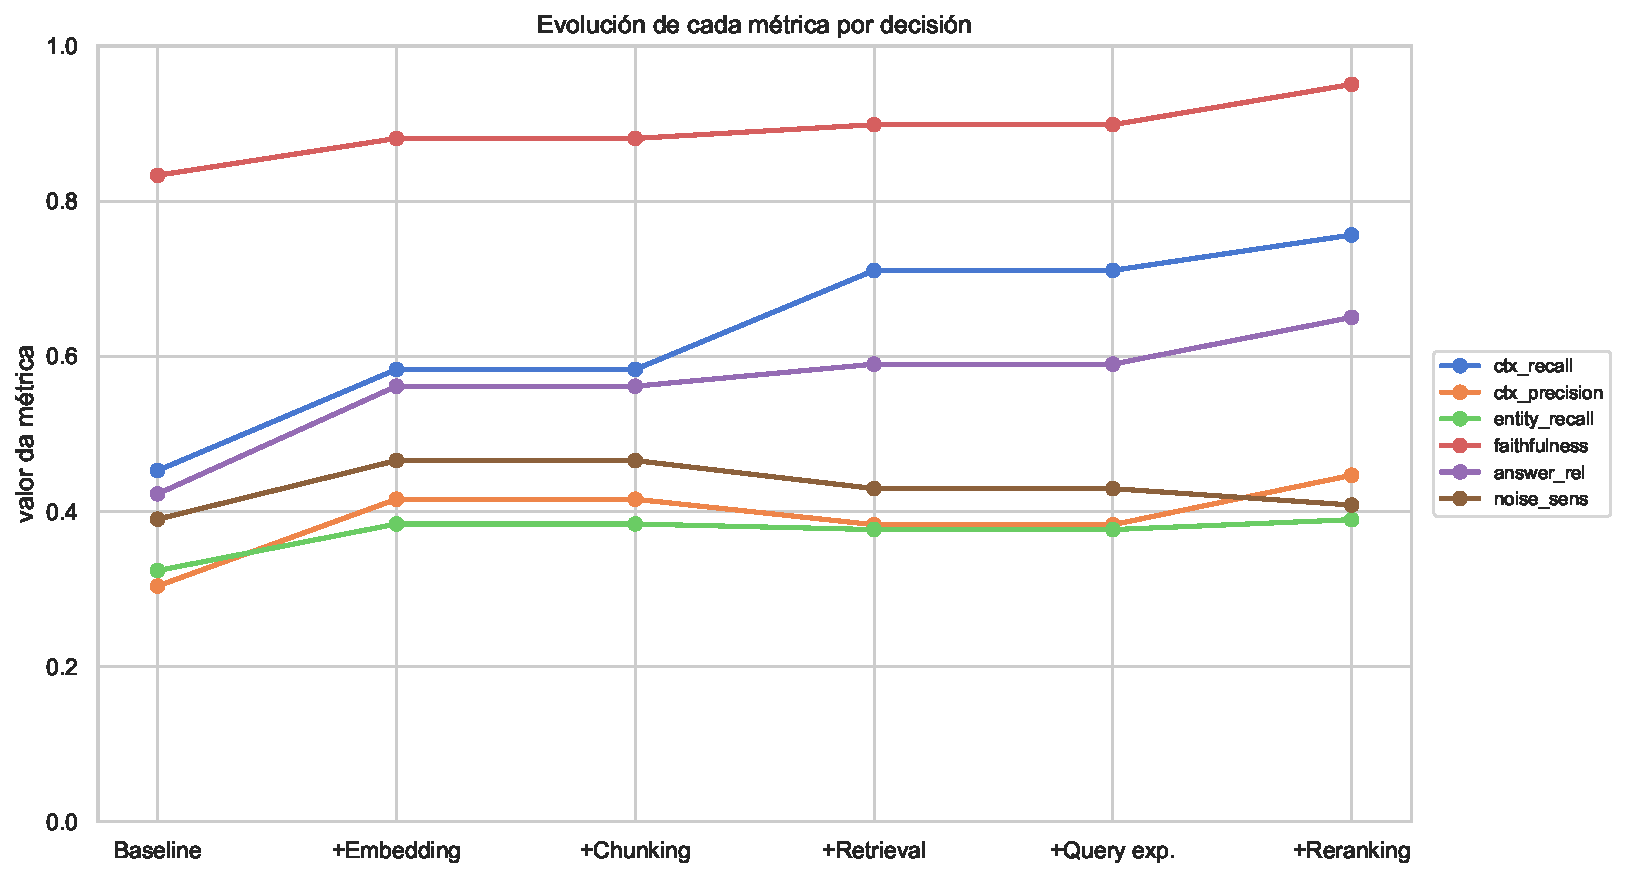
\includegraphics[width=\textwidth]{figures/metrics_evolution}
  \caption{Evolución das seis métricas RAGAS ao longo da ablación}
  \label{fig:res_evolution}
  \fonte{elaboración propia}
\end{figure}

A comparación directa entre o baseline e a pipeline final (Táboa~\ref{tab:res_final})
mostra melloras en todas as métricas de decisión: Context Recall (+0{,}303), Context
Precision (+0{,}143), Faithfulness (+0{,}118) e Response Relevancy (+0{,}227).

\begin{table}[H]
  \centering
  \caption{Baseline fronte á pipeline final óptima}
  \label{tab:res_final}
  \rowcolors{2}{gray!10}{white}
  \footnotesize
  \begin{tabular}{lccccccc}
    \toprule
    \textbf{Configuración} & \textbf{CR} & \textbf{CP} & \textbf{CER} & \textbf{F}
                           & \textbf{RR} & \textbf{NS} & \textbf{P+R} \\
    \midrule
    Baseline (Exp.~0)              & 0,453 & 0,304 & 0,324 & 0,833 & 0,423 & 0,390 & 0,756 \\
    \textbf{Pipeline final (ce k10)} & \textbf{0,756} & \textbf{0,447} & \textbf{0,389} & \textbf{0,951} & \textbf{0,650} & \textbf{0,408} & \textbf{1,203} \\
    \bottomrule
  \end{tabular}
  \fonte{elaboración propia}
\end{table}

\subsection{Validación contra un \textit{stack} estado da arte}
\label{sec:res_sota}

Finalmente, a pipeline óptima compárase cun \textit{stack} maximalista que combina a
técnica máis avanzada sobre o papel de cada dimensión —\texttt{Qwen3-Embedding-8B},
chunking semántico, recuperación híbrida, RAG-Fusion e reranking listwise por LLM—
(Táboa~\ref{tab:res_sota}, Figura~\ref{fig:res_sota}). O resultado valida o enfoque
empírico: a pipeline obtida pola
ablación secuencial (P+R 1{,}203) \textbf{supera} tanto o baseline (0{,}756) como o
\textit{stack} SOTA da literatura (1{,}095), cun mellor Context Precision, Faithfulness e
Response Relevancy. O \textit{stack} SOTA só aventaxa a pipeline empírica en Noise
Sensitivity (0{,}486 fronte a 0{,}408). Isto confirma que a selección empírica de
compoñentes adaptada ao dominio supera a aplicación directa de técnicas xenéricas
consideradas estado da arte.

\begin{table}[H]
  \centering
  \caption{Pipeline empírica fronte ao \textit{stack} SOTA da literatura}
  \label{tab:res_sota}
  \rowcolors{2}{gray!10}{white}
  \footnotesize
  \begin{tabular}{lccccccc}
    \toprule
    \textbf{Configuración} & \textbf{CR} & \textbf{CP} & \textbf{CER} & \textbf{F}
                           & \textbf{RR} & \textbf{NS} & \textbf{P+R} \\
    \midrule
    Naive RAG (Exp.~0)         & 0,453 & 0,304 & 0,324 & 0,833 & 0,423 & 0,390 & 0,756 \\
    Stack SOTA (literatura)    & 0,708 & 0,387 & 0,354 & 0,869 & 0,566 & 0,486 & 1,095 \\
    \textbf{Pipeline empírica} & \textbf{0,756} & \textbf{0,447} & \textbf{0,389} & \textbf{0,951} & \textbf{0,650} & \textbf{0,408} & \textbf{1,203} \\
    \bottomrule
  \end{tabular}
  \fonte{elaboración propia}
\end{table}

\begin{figure}[H]
  \centering
  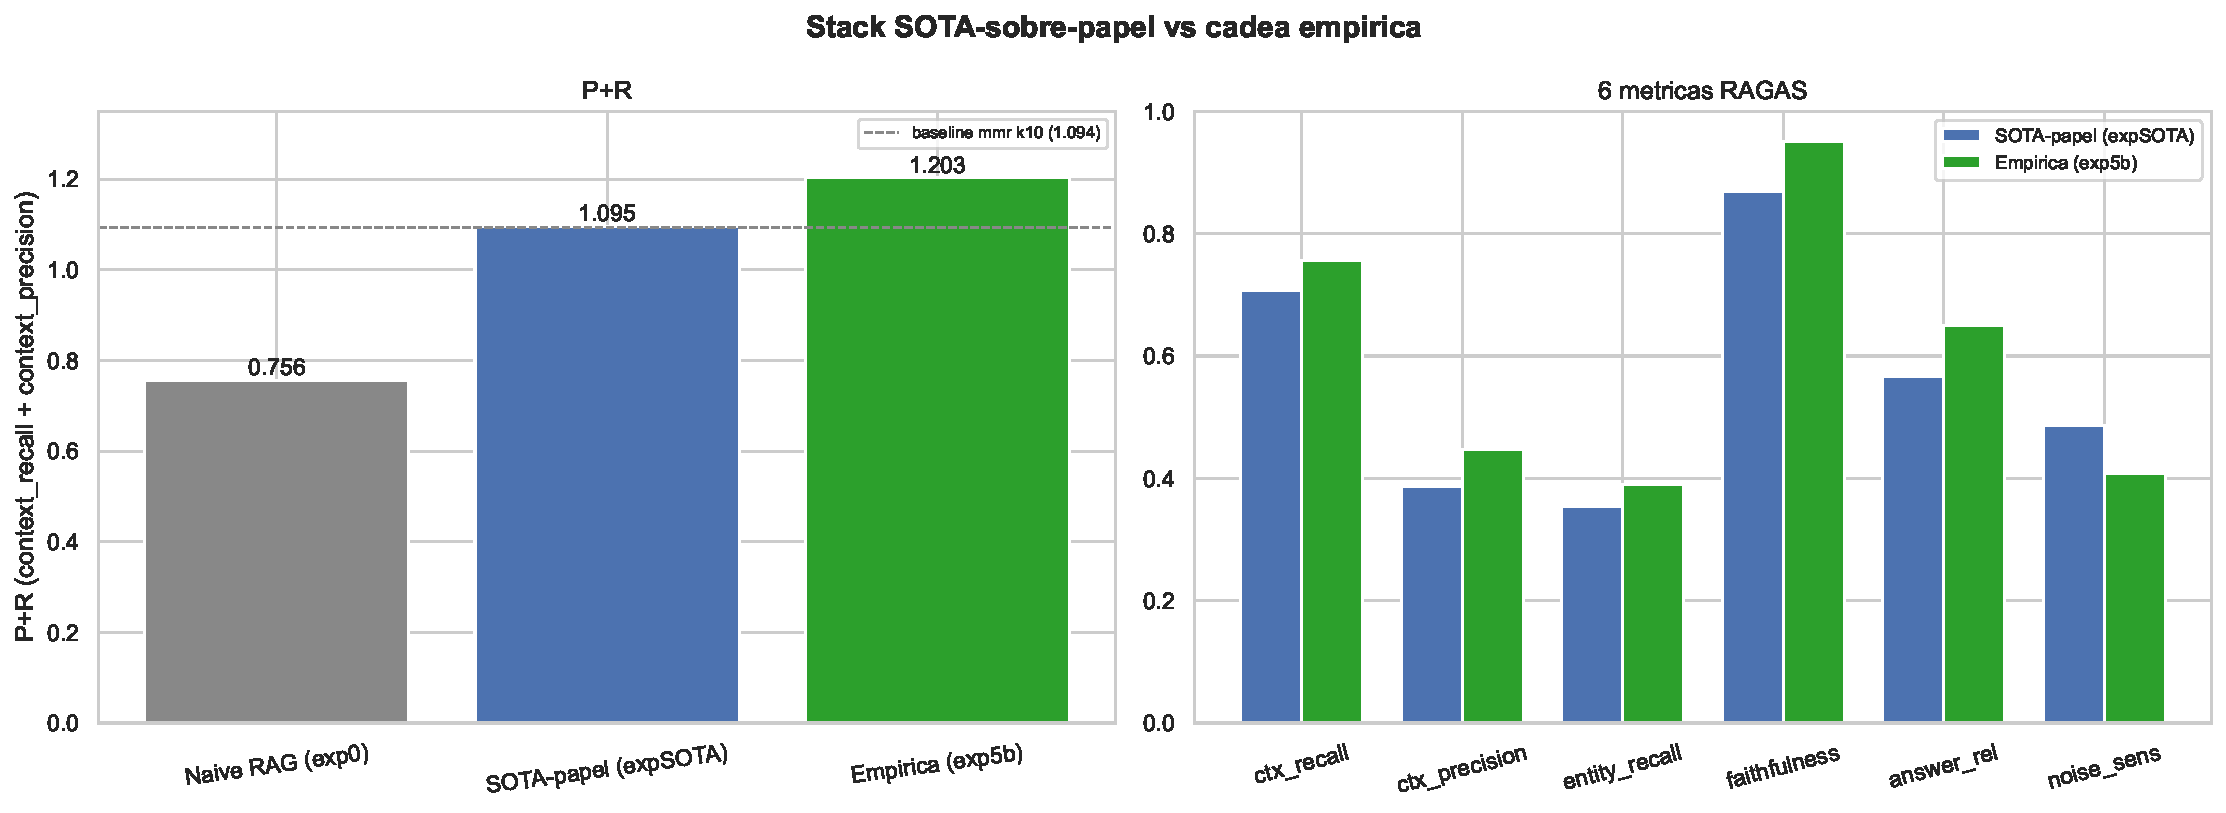
\includegraphics[width=\textwidth]{figures/sota_stack_vs_empirical}
  \caption{Comparación da pipeline empírica co \textit{stack} SOTA e o baseline}
  \label{fig:res_sota}
  \fonte{elaboración propia}
\end{figure}


%% ============================================================
%%  CONCLUSIÓNS E AMPLIACIÓN
%% ============================================================
\chapter*{Conclusións e ampliación}
\addcontentsline{toc}{chapter}{Conclusións e ampliación}
\markboth{Conclusións e ampliación}{Conclusións e ampliación}

\subsection*{Síntese de resultados}

Este traballo abordou a optimización experimental dunha pipeline RAG sobre o corpus
xurídico EUR-Lex mediante unha ablación secuencial de cinco fases, avaliada con seis
métricas RAGAS sobre un golden dataset de 149 pares pregunta--resposta. A configuración
final óptima —embedding \texttt{bge-m3}, chunking fixo de 256~tokens, recuperación
\texttt{mmr} con $k = 10$, sen expansión de consultas e reranking con cross-encoder
\texttt{bge-reranker-v2-m3} ($k = 10$)— elevou a métrica agregada de recuperación P+R
desde 0{,}756 (baseline Naive RAG) até 1{,}203, unha mellora relativa do 59\,\%, e
superou tamén a un \textit{stack} que combina técnicas estado da arte da literatura
(P+R 1{,}095).

As preguntas de investigación respóndense do seguinte xeito:

\begin{description}
  \item[\textbf{RQ1}:] O modelo \texttt{bge-m3} é o que mellor representa o corpus
    EUR-Lex, cunha mellora de +0{,}243 en P+R sobre o baseline —a maior decisión
    individual de toda a ablación—. O tamaño do modelo non é determinante: o moito maior
    \texttt{qwen3-embedding-8b} obtivo peores resultados.
  \item[\textbf{RQ2}:] Ningunha estratexia de chunking avanzada superou o chunking fixo
    de 256~tokens. A segmentación estrutural, a priori axeitada para documentos
    xurídicos, resultou a peor opción, polo que se mantivo o chunking fixo.
  \item[\textbf{RQ3}:] A diversificación \ac{MMR} con $k = 10$ mellorou de forma
    consistente a recuperación densa (+0{,}095 en P+R). A recuperación esparsa (BM25) e
    a híbrida non superaron a densa neste dominio.
  \item[\textbf{RQ4}:] Ningunha das sete técnicas de expansión de consultas mellorou a
    base; en cambio, o reranking con cross-encoder ($k = 10$) foi a segunda mellora máis
    importante (+0{,}109 en P+R), superando ao reranking listwise por LLM cun custo
    computacional moi inferior.
  \item[\textbf{RQ5}:] A pipeline construída empiricamente mediante a ablación secuencial
    superou o \textit{stack} de técnicas estado da arte da literatura, o que confirma
    que a selección de compoñentes adaptada ao dominio é máis eficaz que a aplicación
    directa de técnicas xenéricas.
\end{description}

\subsection*{Implicación metodolóxica}

Máis alá das configuracións concretas gañadoras, o achado transversal deste traballo é
de natureza metodolóxica: \textbf{non existe unha única receita correcta para construír
unha pipeline RAG}. A configuración óptima depende do dominio, da natureza dos documentos
e do tipo de consultas, e só pode determinarse de forma empírica. Esta afirmación non é
unha intuición, senón que se sostén directamente sobre a evidencia recollida ao longo da
ablación:

\begin{itemize}
  \item O \textit{stack} que combina as técnicas consideradas estado da arte na
    literatura —o que cabería esperar como \enquote{a forma correcta} de facelo— foi
    superado pola pipeline axustada empiricamente fase a fase (P+R 1{,}095 fronte a
    1{,}203).
  \item Decisións aparentemente axeitadas para o dominio fallaron: a segmentación
    estrutural, deseñada para aproveitar a organización por artigos dos textos xurídicos,
    resultou a peor estratexia de chunking.
  \item Técnicas amplamente recomendadas non aportaron ningunha mellora: ningunha das
    sete técnicas de expansión de consultas superou a base.
  \item O tamaño non garante o rendemento: o modelo de embedding máis grande
    (\texttt{Qwen3-Embedding-8B}, 8.000~M de parámetros) foi superado por un modelo moito
    máis pequeno (\texttt{bge-m3}).
\end{itemize}

En consecuencia, a principal recomendación práctica deste traballo é que a única forma
correcta de optimizar un sistema RAG é probalo empiricamente sobre o dominio concreto de
aplicación: a optimización debe abordarse sempre como un proceso experimental e medido,
en lugar de asumir que as técnicas máis avanzadas ou de maior tamaño producirán por si
soas os mellores resultados. Esta conclusión é coherente coa marcada variabilidade do
rendemento dos sistemas RAG entre dominios sinalada na literatura
\citep{gao2023retrieval}.

\subsection*{Contribución instrumental e aplicabilidade}

A implicación anterior outorga un valor especial ao segundo resultado deste traballo, de
natureza instrumental. Se a configuración óptima dun sistema RAG non é universal e debe
determinarse empiricamente en cada dominio, entón o activo máis duradeiro non son os
gañadores concretos —que envellecen a medida que aparecen novos modelos— senón o
\textbf{marco experimental reproducible} construído para obtelos. Este traballo materializa
ese marco como unha infraestrutura parametrizable (implementada con Kedro,
Sección~\ref{sec:kedro}) na que cada experimento se define por configuración, é
reproducible e auditable, e na que substituír o corpus, o modelo de embedding ou calquera
outro compoñente non require reescribir código, senón cambiar parámetros.

Esta separación entre lóxica e configuración converte o marco nun entregable reutilizable
con aplicabilidade directa en contornos profesionais: calquera organización que dispoña
dun corpus documental propio pode empregalo para identificar, de forma sistemática e
medida, a configuración RAG máis axeitada ao seu dominio antes de levala a produción, e
re-executalo periodicamente a medida que evolucionan os modelos dispoñibles. Deste xeito,
a contribución do traballo non se limita a un resultado empírico puntual sobre EUR-Lex,
senón que ofrece un método e unha ferramenta transferibles para a toma de decisións
tecnolóxicas no deseño de sistemas RAG.

\subsection*{Limitacións do estudo}

O presente estudo presenta as seguintes limitacións que deben terse en conta ao
interpretar os resultados:

\begin{itemize}
  \item \textbf{Dominio único.} Os experimentos realízanse exclusivamente sobre
    documentos xurídicos europeos. A xeneralización dos resultados a outros dominios
    (médico, financeiro, científico) non está garantida.
  \item \textbf{Custo computacional de RAGAS.} A avaliación con RAGAS require múltiples
    chamadas ao LLM por exemplo, o que implica un custo económico e limita o número
    de configuracións avaliables.
  \item \textbf{Dependencia do modelo avaliador.} RAGAS usa un LLM como xuíz, polo que
    os resultados das métricas están parcialmente condicionados pola calidade e os
    nesgos do modelo empregado para a avaliación.
  \item \textbf{Golden dataset limitado.} O tamaño do conxunto de avaliación está
    limitado polo custo de construción manual. Conxuntos de maior tamaño poderían
    reducir a varianza nas estimacións das métricas.
  \item \textbf{Alcance das arquitecturas avaliadas.} O estudo céntrase na optimización
    dos compoñentes dunha pipeline RAG estándar (embedding, chunking, retrieval,
    expansión de consultas e reranking). As arquitecturas que modifican o fluxo completo
    do sistema (CRAG, Adaptive-RAG, RAG axéntico, GraphRAG) quedaron fóra do alcance
    experimental polo seu elevado custo de implementación e execución, e propóñense como
    traballo futuro.
  \item \textbf{Optimización greedy.} A ablación secuencial non garante un óptimo global:
    posibles interaccións entre compoñentes (por exemplo, entre embedding e chunking)
    poderían facer que outra combinación non explorada superase a obtida. Avaliar
    exhaustivamente o produto cartesiano de todas as opcións consideradas en cada fase
    —catro modelos de embedding, seis estratexias de chunking, oito configuracións de
    retrieval, oito de expansión de consultas e cinco de reranking— implicaría arredor
    de 7.680 combinacións ($4 \times 6 \times 8 \times 8 \times 5$), cada unha cun custo
    de avaliación RAGAS proporcional ao tamaño do golden dataset. Tal busca exhaustiva é
    computacionalmente inviable, polo que a ablación secuencial —que reduce o problema a
    unhas poucas decenas de configuracións (arredor de 25)— constitúe un compromiso
    necesario entre exhaustividade e custo.
\end{itemize}

\subsection*{Traballo futuro}

Este traballo abre varias liñas de investigación futura:

\begin{itemize}
  \item Extensión do benchmark a outros dominios especializados (medicina, finanzas)
    para contrastar a xeneralizabilidade dos resultados obtidos en EUR-Lex.
  \item Estudo do impacto de modelos de embedding específicos do dominio xurídico
    (\textit{fine-tuned} sobre corpus legal) sobre as métricas de recuperación, máis
    alá dos modelos de propósito xeral avaliados neste traballo.
  \item Avaliación de arquitecturas RAG que modifican o fluxo completo do sistema
    —Self-RAG, RAG correctivo (CRAG), Adaptive-RAG, RAG axéntico con LangGraph e
    GraphRAG— sobre a pipeline óptima obtida neste traballo, para comprobar se superan
    ao mellor RAG base.
  \item Avaliación de estratexias de recuperación iterativa activa como FLARE, que
    decide adaptativamente cando xerar e cando recuperar información adicional.
  \item Construción dun golden dataset de maior tamaño mediante anotación humana
    sistemática, co obxectivo de reducir a varianza nas estimacións das métricas e
    permitir análises estatísticas máis robustas.
  \item Análise do impacto do modelo LLM xerador sobre os resultados, comparando
    modelos de código aberto con modelos de propósito xeral para identificar opcións
    economicamente viables en produción.
  \item Evolución do marco experimental cara a unha ferramenta de produción completa:
    despregamento do sistema RAG óptimo como servizo (API e interface de usuario),
    medición de latencia e custo en operación real, e integración do proceso de
    optimización nun fluxo de \textit{MLOps} que permita reavaliar a configuración de
    forma automática a medida que evolucionan os modelos e o corpus.
\end{itemize}

%% ============================================================
%%  BIBLIOGRAFÍA
%% ============================================================
\printbibliography[heading=bibintoc, title={Bibliografía}]

\end{document}
